\chapter{Serial Verbs} \label{ch:sv}

In this section I will introduce what I mean when I refer to serial verb constructions (SVCs) in Nuuchahnulth (\S\ref{ch:sv:def}), give the data on the construction (\S\ref{ch:sv:data}), and finally my analysis as implemented in my grammar (\S\ref{ch:sv:analysis}).

\section{Serial Verb Definition} \label{ch:sv:def}

To investigate the properties of serial verb constructions (SVCs) in Nuuchahnulth I first have to define what I count as such a construction in the language. I will here give my reasoning for the definition, and what I exclude from the category.

It is difficult to find a single widely accepted definition of serial verbs in the linguistic literature. Even in their typological survey, \cite{aikhenvalddixon2006} give several definitions, some of which conflict with each other. They define SVCs as multiple verbs that (i) are monoclausal; (ii) from a ``single predicate"; (iii) form a ``single event"; (iv) form one unit phonologically; (v) are negated singly. Most of these definitions are problematic or vague. \citeauthor{aikhenvalddixon2006} give no clear definition for a single predicate or a single event. Without a formal semantic representation, these are left vague, and the definition of a single predicate (when it is not synonymous with a single event) seems to come down to monoclausality. While serial verbs may be phonologically connected, they give several examples where the serial verbs are separated by intervening words (such as a direct object), and give instances of serial verbs (on their definition) where one verb is negated while the other is not. So none of these definitional properties are necessary, and those that are are underdefined. This is perhaps necessary when trying to define a phenomenon across all of human language.

I am only looking at one language, Nuuchahnulth, and will tailor my definition of a serial verb construction to the language, while attempting to keep the definition as broadly applicable as possible. I will avoid making claims about ``single predicates" and ``single events" without defining those terms within an analytical framework (\S\ref{ch:sv:def:compositionality}). My functional definition of a serial verb construction in Nuuchahnulth is this:

\ex \label{svcdef}
Any clause containing two verbs without an overt coordinator, and where the verbs share the semantic interpretation of the second position clausal inflection is a serial verb construction.
\xe

Each matrix and dependent clause is marked with a second-position clitic, and so the boundaries of a clause are often easy to determine. The one exception to this is that the third-person neutral mood is null-marked. For this reason, I will use examples that are not in this person-mood combination. Because of the restriction that serial verb constructions lack an overt coordinator, constructions containing a linker morpheme (\S\ref{ch:link}) do not count as SVCs.

The requirement of sharing the second position clausal inflection is clearly Nuuchahnulth-specific. However, it is a way to capture the distinction between a single clause with a serial verb construction and two separate clauses. The way to determine a clause boundary will differ language to language. Because clause boundaries in Nuuchahnulth include subject information, the verbs necessarily share a subject. This may be true of all SVCs, but I make no such claim here. Importantly, this definition says nothing about the semantics or event properties of a SVC, only that a serial verb construction is one where verbs relate to one another within the limits of a clause. There is room for a great deal of difference and diversity of SVCs that meet this definition, and this is by design.

%This definition is also restricted to verbs, and not other kinds of multi-predicate constructions. Non-verbs do not participate in the kinds of constructions I will investigate here, and non-verbal multi-predicate constructions are fairly limited in type: they require overt coordination through a coordinand or through a linker construction. The former is outside the scope of this dissertation, and the latter will be addressed in \S\ref{ch:link}.

\subsection{Semantic Compositionality} \label{ch:sv:def:compositionality}

I have an analytical preference for semantic compositionality where possible. Semantic compositionality means that one can create the semantics of the sentence directly from the semantics of lexical items and combinatoric rules in the syntax. In my analysis (\S\ref{ch:sv:analysis}) I will be able to maintain compositionality for Nuuchahnulth SVCs. This may be a result of the facts about Nuuchahnulth as well as my framework, and I make no claims about semantic compositionality in SVCs cross-linguistically.

As an example of an SVC analysis that does not maintain compositionality, I will use \cite{butt1995}'s analysis of Urdu serial verbs.  A key component of \citeauthor{butt1995}'s analysis is the notion of a ``complex predicate," which is the creation of a new atomic unit of meaning from two separate words. The two components of a complex predicate may have a hierarchical relation in the syntax of the language (which contradicts the monoclausality requirement of \cite{aikhenvalddixon2006}), but form a new semantic unit. The semantic relation for the word `write' might be \textsc{write}(\textit{x}, \textit{y}), but when combined with the Urdu permissive verb \textsc{let}(\textit{a},\textsc{b}), the new semantic relation is \textsc{let-write}(\textit{x}, \textit{y}, \textit{z}). The composed semantic relation in this case has a different number of arguments from either of its dependent relations.

Despite the apparent relationship between \textsc{write}, \textsc{let}, and \textsc{let-write}, this analysis, without the development of a fuller semantic formalism, violates semantic compositionality. We write a relation and its elementary predication with upper-case letters as a shorthand for the `meaning' of that morpheme. However, this convention is only for human readability, since we are not actually defining what those units mean but just using them as placeholders for ``whatever the proper lexical semantics are." We could define the meaning of \textit{write} as \textsc{meaning1647} with no loss of specificity. \citeauthor{butt1995}'s analysis creates a situation where there is a new mathematical operation in the semantic representation: `let' \textsc{let} + `write' \textsc{write} = \textsc{let-write}. Despite the similarity in labels, there is no formal relationship between these three meaning representations except by that equation. It is just as though the equation had been \textsc{meaning1647} + \textsc{meaning2119} = \textsc{meaning8780}. Even though the meaning of Urdu's \textit{let-write} is semantically compositional in the language, the meaning representation of \citeauthor{butt1995}'s ``complex predicate" in the formalism is non-compositional with respect to its members.

This is not necessarily a bad thing in all contexts. Some sort of arbitrariness is necessary when modeling multi-word expressions like idioms, which have for a long time been understood as not fully compositional \citep{chafe1968}, although multi-word expressions can vary in their semantic compositionality \citep{nunberg1994}. It is possible that many SVCs are not-quite compositional and a non-compositional semantic relation is an appropriate model. However, when this kind of rule is productive and has predictable semantics (as in the case for SVCs in Nuuchahnulth), I believe it is preferable to adhere to semantic compositionality in the formal analysis. Otherwise, one ends up with a list of semantic equations which is nearly the size of the set of verbs in the lexicon, if not larger.

In Lexical-Functional Grammar (LFG), which is the framework that \citeauthor{butt1995} uses, the elementary predication (the all-caps semantic relation) of a word is linked to the number of its arguments. That is, the meaning of `write' isn't merely \textsc{write}, but \textsc{write}(\textit{x}, \textit{y}). In LFG then, to add an argument to a relation, it is necessary to change the relation's meaning itself, and this is what \citeauthor{butt1995} does. In MRS \citep{copestake2005}, the elementary predication and its arguments are separated from each other. That is, the meaning of `write' is represented as:

\ex
\begin{avm}
\[ pred & \textsc{write} \\
   arg0 & \textit{e} \\
   arg1 & \textit{x} \\
   arg2 & \textit{y} \\
\]	
\end{avm}
\xe

This separability is something the formalism shares with Neodavidsonian representations \citep{parsons1990}, and will allow me to maintain strict semantic compositionality in my analysis of serial verbs in Nuuchahnulth.

\subsection{Non-SVCs}

I have defined Nuuchahnulth serial verb constructions in (\ref{svcdef}) as any clause (defined by the second position clausal enclitics) which contains more than one verb, without any overt coordinator, and where the clausal enclitics are semantically interpreted as belonging to all verbs in the construction. There are a few types of constructions that nearly fit this definition, but are excluded. The first is juxtaposed clauses (\ref{ex:juxtaposedclauses}).

\ex \label{ex:juxtaposedclauses}
\begingl
\glpreamble hač̓a pawałšiƛ [pause] ʔuušp̓iq [pause] ʔuušp̓iqqač̓a wawaa. //
\gla hač̓a pawał-šiƛ ʔuušp̓iq ʔuušp̓iq=qaˑč̓a wawaa. //
\glb maybe lost-\textsc{mo} something.bad.happens.\textsc{mo} something.bad.happens.\textsc{mo}=\textsc{dubv} say.\textsc{cv} //
\glft ` ``Maybe he got lost... something happened... perhaps something happened," they said.' (\textbf{C}, \textit{tupaat} Julia Lucas) //
\endgl
\xe

(\ref{ex:juxtaposedclauses}) comes from a text about a man who was lost at sea and returns. Although one could claim that the first two verbs, \textit{pawałšiƛ} and \textit{ʔuušp̓iq}, are in a SVC, the prosody used in the utterance indicates something else. The repeated \textit{ʔuušp̓iq}, complete with a second position clitic, suggests that these are clauses (the first two under null-marked third person neutral mood) that are adjacent. This kind of structure occurs in speech as people are rephrasing or redescribing an event. (\ref{ex:juxtaposedclauses2}) has the same structure, and is from a description of Raven in a narrative text.

\ex \label{ex:juxtaposedclauses2}
\begingl
\glpreamble ʔayiisšiƛ, hiy̓iisšiƛ haʔumukʔi. //
\gla ʔaya-!iis-šiƛ hiš-!iis-šiƛ haʔum=uk=ʔiˑ //
\glb many-consume-\textsc{mo} all-consume-\textsc{mo} food=\textsc{poss}=\textsc{art} //
\glft `He ate a lot, he ate all of the food.' (\textbf{B}, Marjorie Touchie) //
\endgl
\xe

Like (\ref{ex:juxtaposedclauses}), (\ref{ex:juxtaposedclauses2}) is in the third person, and I believe this is two separate clauses, and not a serialization structure. When these sorts of constructions occur outside the third person, the adjacent clauses require an overt enclitic, and so this apparent ambiguity (serialization vs adjacent clause) does not occur.

The second kind of construction that falls outside my definition of a SVC is temporal expressions. The way to express a duration of time is to juxtapose the time period with the rest of the clause. If the time expression is in the durative aspect, the interpretation is `for \textit{x} time' (\ref{ex:inportforfivedays}). If the time expression is in a perfective aspect, the interpretation is `after \textit{x} time' or `at the end of \textit{x} time' (\ref{ex:afterayear}).

\ex \label{ex:inportforfivedays}
\begingl
\glpreamble suč̓ačłintiis hił c̓uumaʕaas. //
\gla suč̓a-čiˑł=int=(y)iis hił c̓uumaʕaas //
\glb five-day.\textsc{dr}=\textsc{pst}=\textsc{weak.1sg} be.at Port.Alberni //
\glft `I was in Port Alberni for five days.' (\textbf{Q}, Sophie Billy) //
\endgl
\xe

\ex~ \label{ex:afterayear}
\begingl
\glpreamble ʔaḥʔaaʔaƛqač̓a n̓upqʔičḥšiʔeƛ n̓aacsaaƛ ḥiškʷiiʔatḥ č̓apac hintšiƛ ʔuucay̓uk ḥiškʷiiʔatḥ. //
\gla ʔaḥʔaaʔaƛ=qaˑč̓a n̓up-qʔičḥ-šiƛ=!aƛ n̓aacsa=!aƛ ḥiškʷiiʔatḥ č̓apac hintšiƛ ʔu-L.cay̓uk ḥiškʷiiʔatḥ //
\glb and=\textsc{dubv} one-year.\textsc{dr}-\textsc{mo}=\textsc{now} see=\textsc{now} Hesquiaht canoe arrive.\textsc{mo}.\textsc{gr} \textsc{x}-go.\textsc{dr} Hesquiaht //
\glft `And one year later the Hesquiahts saw a boat arriving toward Hesquiaht.' (\textbf{C}, \textit{tupaat} Julia Lucas) //
\endgl
\xe

Although these two types of temporal expression are distinct, it is possible to use the second construction, which uses a perfective form, to express a duration, i.e. \textit{it has become X length of time that Y has been done}, as in \ref{ex:forfourdays}. The opposite (interpreting the durative form to mean `after') is not possible to my knowledge.

\ex \label{ex:forfourdays}
\begingl
\glpreamble ʔaḥʔaaʔaƛ muučiiłšiƛna hił siy̓a ʔaḥʔaaʔaƛ ḥaakʷaaƛuk Matthew, kʷaaʔuucukqs. //
\gla ʔaḥʔaaʔaƛ muu-čiˑł-šiƛ=naˑ hił siy̓a ʔaḥʔaaʔaƛ ḥaakʷaaƛ=uk Matthew kʷaaʔuuc=uk=qs //
\glb and four-day.\textsc{dr}-\textsc{mo}=\textsc{neut.1pl} be.at \textsc{1sg} and young.girl=\textsc{poss} Matthew grandchild=\textsc{poss}=\textsc{defn.1sg} //
\glft `We were there for four days, me and Matthew's daughter, my granddaughter.' (\textbf{C}, \textit{tupaat} Julia Lucas) //
\endgl
\xe

What differentiates these expressions from serial verb constructions, as well as linker constructions (see \S\ref{ch:link}) is the interpretation of the subject. While the temporal component can take the subject-mood portmanteau (\ref{ex:inportforfivedays}, \ref{ex:forfourdays}), the person expressed in the subject clitic is not in any way the subject of the temporal expression. In (\ref{ex:inportforfivedays}), `I' is not the subject of `five days.' This is also the case for the subjects of the verbs in (\ref{ex:afterayear}, \ref{ex:forfourdays}). Instead, the time expression seems to be opaque to the subject information present in the clause. So while this construction does have two verbs in a single clause, the interpretive scope of the second position enclitics only falls on one of the verbs (the non-temporal one), and this type of construction is excluded from my scope for serial verbs.

\section{Data} \label{ch:sv:data}

\subsection{Types of Serial Verb Constructions}

Descriptively, I have categorized observed serial verb constructions into four types. These types are not motivated a priori by any external typological theories or a commitment to these categories, but an attempt to make sense of my data, and in my analysis (\S\ref{ch:sv:analysis}) I will collapse Types I-III into the same analytical type, but I leave them separated here in an attempt to maintain a distinction between data and analysis.

\vspace{10pt}

\subsubsection{Type I: Simultinaeity} \label{ch:sv:data:type1}

\vspace{10pt}

This SVC links two verbs together that necessarily occur simultaneously. Semantically, they can often be described loosely as ``manner and action"---where one verb is expressing the main action, and another is expressing how it is done. This includes motion and manner of motion (e.g., go + walk as in \ref{ex:walktoalberni}), a semantically light verb like ``do" coordinating with the actual action (e.g., only-do + lie-down as in \ref{ex:justliedown}), and metaphoric motion and action (e.g., go-back + become-alive as in \ref{ex:comebacktolife}).

\ex \label{ex:walktoalberni}
\begingl
\glpreamble \textbf{ʔuucuʔuk}w̓it̓asaḥ \textbf{yaacuk} c̓uumaʕas. //
\gla \textbf{ʔuucuʔuk}-w̓it̓as=(m)aˑḥ \textbf{yaacuk} c̓uumaʕas //
\glb \textbf{go.to.\textsc{dr}}-going.to=\textsc{real.1sg} \textbf{walk.\textsc{dr}} Port.Alberni //
\glft `I'm going to walk to Port Alberni.' (\textbf{B}, Bob Mundy) //
\endgl
\xe

\ex~ \label{ex:justliedown}
\begingl
\glpreamble \textbf{ʔanasł}intwaʔš \textbf{t̓awiłšƛ}. //
\gla \textbf{ʔana-siła}=int=waˑʔš \textbf{t̓awił-šiƛ} //
\glb \textbf{only-do}=\textsc{pst}=\textsc{hrsy.3} \textbf{lie.down-\textsc{mo}} //
\glft `He just laid down.' (\textbf{Q}, Sophie Billy) //
\endgl
\xe

\begin{comment}
\ex~ \label{ex:goaheadwent}
\begingl
\glpreamble nay̓iiʔak̓aƛin \textbf{kuw̓iła} \textbf{wałaak}. //
\gla nay̓iiʔak=!aƛ=(m)in \textbf{kuw̓iła} \textbf{wałaak} //
\glb immediately=\textsc{now}=\textsc{real.1pl} \textbf{go.ahead} \textbf{go.to.\textsc{dr}} //
\glft `We immediately went ahead and went.' (\textbf{B}, Marjorie Touchie) //
\endgl
\xe
\end{comment}

\ex~ \label{ex:comebacktolife}
\begingl
\glpreamble \textbf{huʔacači}ʔaqƛsuuk \textbf{tiičačiƛ}. //
\gla \textbf{huʔa-ca-čiƛ}=!aaqƛ=suuk \textbf{tiič-°ačiƛ} //
\glb \textbf{back-go-\textsc{mo}}=\textsc{fut}=\textsc{neut.2pl} \textbf{live-\textsc{in}} //
\glft `You will come back to life.' (\textbf{C}, \textit{tupaat} Julia Lucas) //
\endgl
\xe

However, this construction is not limited to the semantics of ``manner and motion." Speakers can also coordinate verbs that describe resultative and simultaneous actions (e.g., feel sorry for + mistreat as in \ref{ex:dontmistreatme}), or what I sometimes call serial repetition, which includes cases where a transitive and intransitive verb are both used to express an action (e.g., eat + eat in \ref{ex:eateat}, and cry + cry for in \ref{ex:crycry}), or where two transitive verbs, one more specific and less specific, are used (e.g., say + talk about in \ref{ex:sayabout}). The only unifying property of these SVCs seems to be simultaneity.

\ex \label{ex:dontmistreatme}
\begingl
\glpreamble wik̓iis \textbf{x̣ax̣aał} \textbf{łaakʷiił} siy̓a. //
\gla wik=!iˑs \textbf{x̣ax̣aał} \textbf{łaakʷiił} siy̓a //
\glb \textsc{neg}=\textsc{cmmd.2sg>1sg} \textbf{feel.sorry} \textbf{mistreat} \textsc{1sg} //
\glft `Don't feel sorry for me, mistreating me.' (\textbf{C}, \textit{tupaat} Julia Lucas) //
\endgl
\xe

\ex~ \label{ex:eateat}
\begingl
\glpreamble ʔu\textbf{ʔiic̓}aʔaƛ̓ \textbf{haʔuk}. //
\gla ʔu-\textbf{!iic}=!aƛ=!iˑ \textbf{haʔuk} //
\glb \textsc{x}-\textbf{eat.\textsc{dr}}=\textsc{now}=\textsc{cmmd.2sg} \textbf{eat} //
\glft `Eat it!' (\textbf{Q}, Sophie Billy) //
\endgl
\xe

\ex~ \label{ex:crycry}
\begingl
\glpreamble \textbf{ʕiḥak}itʔiš \textbf{ʔuʔuuy̓uk}\footnotemark\ ʔumʔiiqsakʔi. //
\gla \textbf{ʕiḥ-ak}=(m)it=ʔiˑš \textbf{ʔuʔuuy̓uk} ʔumʔiiqsu=ʔak=ʔiˑ //
\glb \textbf{cry-\textsc{dr}}=\textsc{pst}=\textsc{strg.3} \textbf{cry.for} mother=\textsc{poss}=\textsc{art} //
\glft `She cried for her mother.' (\textbf{C}, \textit{tupaat} Julia Lucas) //
\endgl
\xe

\footnotetext{This is not the normal form of the verb `cry for' which is \textit{ʔuʔuuyuk}. Compare with \textit{-RL.ayuk} in \cite[317]{sapir1939}.}

\ex~ \label{ex:sayabout}
\begingl
\glpreamble \textbf{waa}ʔaƛiič \textbf{ʔuumac̓kʷ} ʔuušḥy̓imskqs. //
\gla \textbf{waa}=!aƛ=(y)ii=č \textbf{ʔu-L.mac̓uk} ʔuuš-(q)ḥy̓uˑ-mis=uk=qaˑs //
\glb \textbf{say}=\textsc{now}=\textsc{weak.3}=\textsc{hrsy} \textbf{\textsc{x}-talk.about} some-be.related.or.friends-\textsc{nmlz}=\textsc{poss}=\textsc{defn.1sg} //
\glft `I heard he was talking about my friends or family.' (\textbf{Q}, Sophie Billy) //
\endgl
\xe

This kind of SVC can ``stack" beyond coordinating just two verbs, to at least three (\ref{ex:movebackucluelet}).

\begin{comment}
\ex \label{ex:onlygotostore}
\begingl
\glpreamble \textbf{ʔanasiła}ʔi \textbf{kuw̓iła} \textbf{ʔucačiƛ} makuwił. //
\gla \textbf{ʔana-siła}=!iˑ \textbf{kuw̓iła} \textbf{ʔu-ca-čiƛ} makuwił //
\glb \textbf{only-do}=\textsc{cmmd.2sg} \textbf{go.ahead} \textbf{\textsc{x}-go.to-\textsc{mo}} store //
\glft `Just go to the store.' (\textbf{C}, \textit{tupaat} Julia Lucas) //
\endgl
\xe
\end{comment}

\ex \label{ex:movebackucluelet}
\begingl
\glpreamble \textbf{huʔacačiƛ}w̓it̓asaḥ \textbf{šiiƛuk} \textbf{wałaak} yuułuʔiłʔatḥ. //
\gla \textbf{huʔa-ca-čiƛ}-w̓it̓as=(m)aˑḥ \textbf{šiiƛuk} \textbf{wałaak} yuułuʔiłʔatḥ //
\glb \textbf{back-go-\textsc{mo}}-going.to=\textsc{real.1sg} \textbf{move.house.\textsc{dr}} \textbf{go.to} Ucluelet //
\glft `I'm going to move back to Ucluelet.' (\textbf{B}, Bob Mundy) //
\endgl
\xe

It is possible for one of the verbs and its object (that is, the full VP of one of the serial verbs) to interrupt the other verb and its object, as in (\ref{ex:drivequeenscove}, \ref{ex:eateat2}, \ref{ex:takechildrentochurch}).

\ex \label{ex:drivequeenscove}
\begingl
\glpreamble ʔuuct̓iiḥs$_{\text{v\_1}}$ [ƛiḥaa]$_{\text{v\_2}}$ Queens Cove$_{\text{obj\_1}}$. //
\gla ʔuuct̓iiḥ$_{\text{v\_1}}$=s [ƛiḥ-(y)aˑ]$_{\text{v\_2}}$ Queens Cove$_{\text{obj\_1}}$ //
\glb go.toward.\textsc{dr}=\textsc{strg.1sg} drive-\textsc{cv} Queens Cove //
\glft `I am driving to Queens Cove.' (\textbf{N}, Fidelia Haiyupis) //
\endgl
\xe

\ex \label{ex:eateat2}
\begingl
\glpreamble ʔu\textbf{ʔiis}ʔaƛ̓in \textbf{haʔuk} suuḥaa. //
\gla ʔu-\textbf{!iis}=!aƛ=!in \textbf{haʔuk} suuḥaa //
\glb \textsc{x}-\textbf{eat}=\textsc{now}=\textsc{cmmd.1pl} \textbf{eat.\textsc{dr}} spring.salmon //
\glft `Let's eat spring salmon!' (\textbf{B}, Bob Mundy and Marjorie Touchie) //
\endgl
\xe

\ex~ \label{ex:takechildrentochurch}
\begingl
\glpreamble hiniicintiisʔinł$_{\text{v\_1}}$ [ʔucičƛ$_{\text{v\_2}}$ ciquuwłi$_{\text{obj\_2}}$]$_{\text{vp\_2}}$ t̓aatn̓aʔiskqs$_{\text{obj\_1}}$. //
\gla hina-iic$_{\text{v\_1}}$=int=(y)iis=ʔinł [ʔu-ci-čiƛ$_{\text{v\_2}}$ ciq-uwił=ʔiˑ$_{\text{obj\_2}}$]$_{\text{vp\_2}}$ L.<t>-t̓an̓a=ʔis=uk=qaˑs$_{\text{obj\_1}}$  //
\glb \textsc{empty}-carry=\textsc{pst}=\textsc{weak.1sg}=\textsc{habit} \textsc{x}-go.to-\textsc{mo} pray-building \textsc{pl}-child=\textsc{dim}=\textsc{poss}=\textsc{defn.1sg} //
\glft `I would always take my children to church.' (\textbf{Q}, Sophie Billy) //
\endgl
\xe


\begin{comment}
%The verbs in this type of SVC, for most speakers, must agree in perfectiveness. Nuuchahnulth has a great many verbal aspect markers which follow the root, but they can be broken into two categories: perfective aspect (momentaneous and inceptive) and imperfective aspect (continuative, durative, repetitive, iterative, and graduative). The derivations in (\ref{aspect}) give a simplified view of my understanding of how these aspects are related to each other. Much of this is taken from \cite{davidson2002}, as well as personal correspondence with Davidson, who deserves much credit for working out this system. My understanding of the inceptive as underlyingly continuative + perfective is indebted to Werle.\footnote{Note that this means that the morphology for the continuative and inceptive do not ``stack," unlike the other aspect forms. So momentaneous + graduative is realized as \textit{-šiƛ} and also a long-short template. However continuative + inceptive is simply \textit{-iˑčiƛ}, not *\textit{-(y)aˑ-iˑčiƛ}. In my implementation, I treat the inceptive as a fully separate aspect, although I believe it is conceptually continuous + perfective.} To simplify the graph, I have combined repetitive-perfective, graduative-perfective, and iterative-perfective into a single node, since verbs in this form cannot undergo further aspectual change.

\ex \label{aspect}
\vspace{-20pt}
\xe
\begin{tikzpicture}[sibling distance=10em,
  every node/.style = {shape=rectangle, align=center}]]
\node (root) at (8,4.5) {Root};
\node (mo) at (2,2) {Momentaneous};
\node (ct) at (6,2) {Continuative};
\node (dr) at (8.5,2) {Durative};
\node (rp) at (12,2) {Repetitive};
\node (it) at (15,2) {Iterative};
\node (in) at (2, 0) {Inceptive};
\node (gr) at (5.5, 0) {Graduative};
\node (pf) at (2, -2) {*-Perfective};
\node (*pf) at (15, -2.14) {};
\draw[->] (root) -- (mo) node[midway,fill=white] {-šiƛ};
\draw[->] (root) -- (ct) node[midway,fill=white] {-(y)aˑ};
\draw[->] (root) -- (dr) node[midway,fill=white] {-uk/-L.ḥi};
\draw[->] (root) -- (rp) node[midway,fill=white] {-LR2L.a};
\draw[->] (root) -- (it) node[midway,fill=white] {-LR2L.š};
\draw[->] (mo) -- (gr) node[near start,fill=lightgray] {-LS};
\draw[->] (in) -- (gr) node[near start,fill=lightgray] {-LS};
\draw[->] (ct) -- (in) node[near start,fill=white] {-iˑčiƛ};
\draw[->] (dr) -- (gr) node[midway,fill=white] {-LS};
\draw[->] (gr) -- (pf) node[near end,fill=lightgray] {-šiƛ};
\begin{scope}[on background layer]
\node[bigbox, fit=(ct)(dr)(it)(gr)(*pf), fill=white] (impf) {};
\node[below left] at (impf.north east) {\textit{imperfective aspect}};
\node[bigbox, fit=(mo)(pf), fill=lightgray] (perf) {};
\node[below right] at (perf.north west) {\textit{perfective aspect}};
\draw[->] (rp) -- (pf);
\draw[->] (it) -- (pf);
%\draw[->] (it) to [out=150,in=30] (pf);
\draw[->] (dr) -- (pf);
\end{scope}
\end{tikzpicture}
\ex \label{aspect}
\vspace{-20pt}
\xe

\begin{tikzpicture}[sibling distance=10em,
  every node/.style = {shape=rectangle, align=center}]
\node (root) at (8,4.5) {Root};
\node (mo) at (2,2) {Momentaneous};
\node (ct) at (8,2) {Continuative};
\node (dr) at (10.5,2) {Durative};
\node (rp) at (13,2) {Repetitive};
\node (it) at (15,2) {Iterative};
\node (in) at (4.5,2) {Inceptive};
\node (mo-grad) at (2,0) {moment.-grad.};
\node (in-grad) at (4.5,0) {incept.-grad.};
\node (dr-grad) at (10.5,0) {durative-grad.};
\node (mo-grad-pf) at (2,-2) {mom.-grad.-perf.};
\node (in-grad-pf) at (4.5,-2) {inc.-grad.-perf.};
\node (dr-pf) at (7,-2) {durative-grad.};
\node (dr-grad-pf) at (10.5,-2) {dur.-grad.-perf.};
\node (rp-pf) at (13,-2) {repet.-perf.};
\node (it-pf) at (15,-2) {iter.-perf.};
\draw[->] (root) -- (mo) node[midway,fill=white] {-šiƛ};
\draw[->] (root) -- (ct) node[midway,fill=white] {-(y)aˑ};
\draw[dashed,->] (root) -- (in) node[midway, fill=white] {-iˑčiƛ};
\draw[->] (ct) -- (in);
\draw[->] (root) -- (dr) node[midway,fill=white] {-uk};
\draw[->] (root) -- (rp) node[midway,fill=white] {-LR2L.a};
\draw[->] (root) -- (it) node[midway,fill=white, right] {-LR2L.š};
\draw[->] (mo) -- (mo-grad) node[near start,fill=lightgray] {-LS};
\draw[->] (in) -- (in-grad) node[near start,fill=lightgray] {-LS};
\draw[->] (dr) -- (dr-grad) node[midway,fill=white] {-LS};
\draw[->] (mo-grad) -- (mo-grad-pf) node[near start,fill=white] {-šiƛ};
\draw[->] (in-grad) -- (in-grad-pf) node[near start,fill=white] {-šiƛ};
\draw[->] (dr) -- (dr-pf) node[midway,fill=white] {-šiƛ};
\draw[->] (dr-grad) -- (dr-grad-pf) node[near start,fill=white] {-šiƛ};
\draw[->] (rp) -- (rp-pf) node[midway,fill=white] {-šiƛ};
\draw[->] (it) -- (it-pf) node[midway,fill=white] {-šiƛ};
\begin{scope}[on background layer]
\node[draw=none, fit=(ct)(dr)(it)(dr-grad), fill=white] (impf) {};
\node[above left] at (impf.north east) {\textit{imperfective}};
\node[bigbox, fit=(mo)(in), fill=lightgray] (perf) {};
\node[below right] at (perf.north west) {\textit{perfective}};
\node[bigbox, fit=(mo-grad-pf)(it-pf), fill=lightgray] (perf2) {};
\node[below right] at (perf2.north west) {\textit{perfective}};
%\draw[->] (rp) -- (pf);
%\draw[->] (it) -- (pf);
%\draw[->] (it) to [out=150,in=30] (pf);
%\draw[->] (dr) -- (pf);
\end{scope}
\end{tikzpicture}

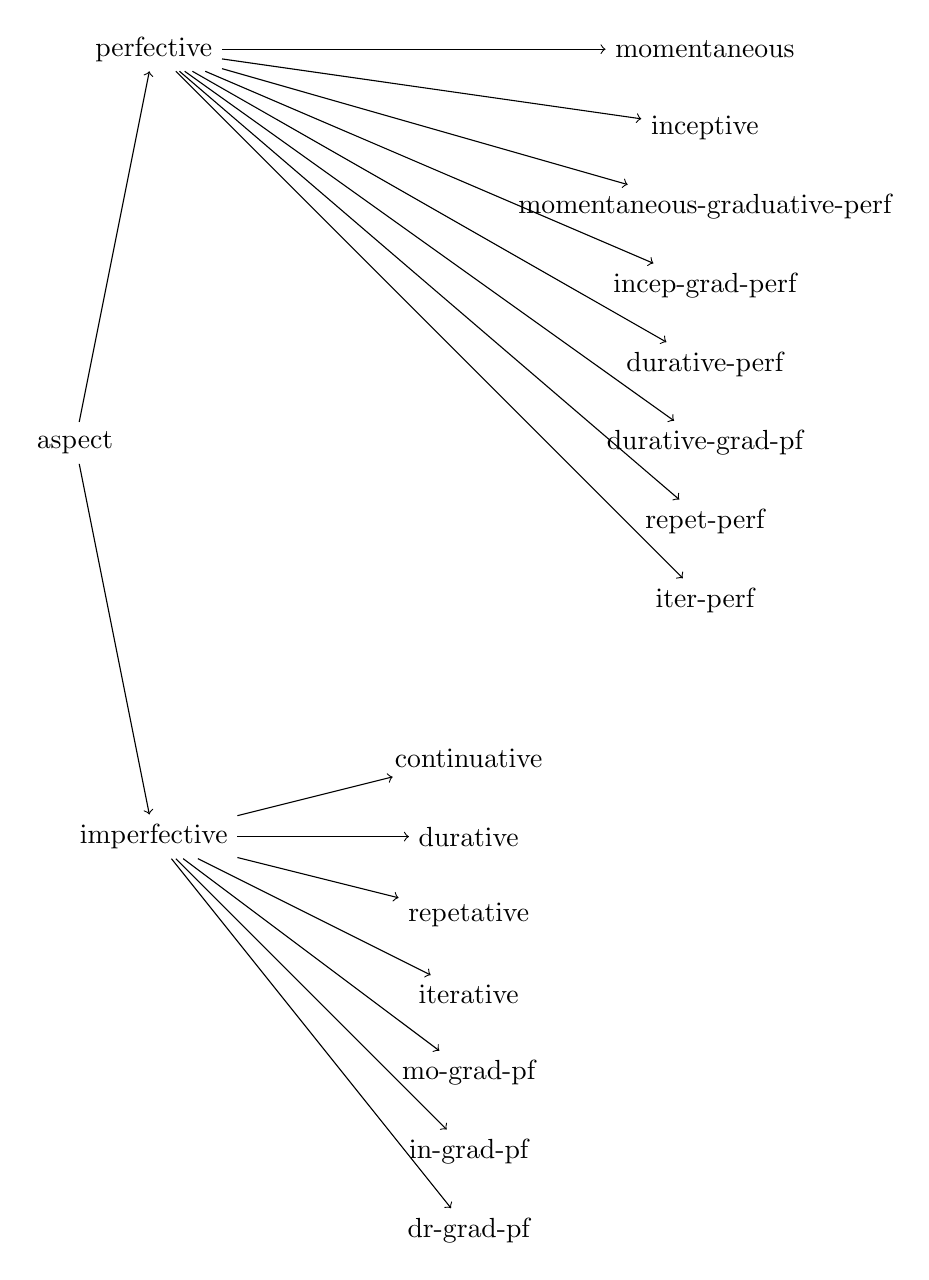
\begin{tikzpicture}[sibling distance=10em,
  every node/.style = {shape=rectangle, align=center}]
\node (aspect) at (0,10) {aspect};
\node (pf) at (1,15) {perfective};
\node (impf) at (1,5) {imperfective};
\node (mo) at (8,15) {momentaneous};
\node (in) at (8,14) {inceptive};
\node (mo-grad-pf) at (8,13) {momentaneous-graduative-perf};
\node (in-grad-pf) at (8,12) {incep-grad-perf};
\node (dr-pf) at (8,11) {durative-perf};
\node (dr-grad-pf) at (8,10) {durative-grad-pf};
\node (rp-pf) at (8,9) {repet-perf};
\node (it-pf) at (8,8) {iter-perf};
\node (ct) at (5,6) {continuative};
\node (dr) at (5,5) {durative};
\node (rp) at (5,4) {repetative};
\node (it) at (5,3) {iterative};
\node (mo-grad) at (5,2) {mo-grad-pf};
\node (in-grad) at (5,1) {in-grad-pf};
\node (dr-grad) at (5,0) {dr-grad-pf};
\draw[->] (aspect) -- (pf);
\draw[->] (aspect) -- (impf);
\draw[->] (pf) -- (mo);
\draw[->] (pf) -- (in);
\draw[->] (pf) -- (mo-grad-pf);
\draw[->] (pf) -- (in-grad-pf);
\draw[->] (pf) -- (dr-pf);
\draw[->] (pf) -- (dr-grad-pf);
\draw[->] (pf) -- (rp-pf);
\draw[->] (pf) -- (it-pf);
\draw[->] (impf) -- (ct);
\draw[->] (impf) -- (dr);
\draw[->] (impf) -- (rp);
\draw[->] (impf) -- (it);
\draw[->] (impf) -- (mo-grad);
\draw[->] (impf) -- (in-grad);
\draw[->] (impf) -- (dr-grad);
\end{tikzpicture}
\end{comment}

%\vspace{10pt}

I noticed in the course of working on this dissertation that this type of SVC have a strong tendency to agree in perfectiveness. For an overview of Nuuchahnulth's aspect system, I refer back to \S\ref{ch:clause:aspect}. Here I will simply say that verb forms that end in the ``inceptive" or ``momentaneous" aspect are perfective, while all other forms are imperfective.

Despite my belief that there is a preference for aspectual matching, speakers were often very flexible on the grammaticality of perfective mismatching when asked about it directly. I made several attempts to suss out whether this was a grammatical rule in one-on-one sessions with speakers, but often received contradicting information. I will first present data from running texts. These texts come from a number of sources: (1) \cite{sapir1939}; (2) Texts gathered by Adam Werle and provided to me (some from speakers I have not worked with and some I have); (3) Texts I elicited with speakers. Some of these were texts I have interlinearized and some I have not.

I went through these texts and marked instances of what I believed to be SVCs. Because a large number of cases in running text are third person, and thus possibly involve more than one clause with a null-marked third person, I had to make educated guesses about whether some third-person constructions were two clauses or a SVC. I used a few tells: (i) the presence or absence of overt (non-neutral) third-person inflection in the surrounding text; (ii) whether the verbs share an (overt) object; (iii) whether the verbs are in an embedded clause. I ranked possible SVCs on a confidence level of 1-4, with 1 being uncertain, 2 a toss-up, 3 likely, and 4 completely positive. I then counted how many times the two verbs in the SVC matched or mismatched in perfectivity. For a few cases (see below) I was uncertain about the perfectivity of one of the verbs and gave it a score of 0.5. I then threw away all SVCs ranked as 1s and 2s. The remaining data are presented in \cref{table:svctype1} below. I have broken this data into five sections: Data from the Nootka Texts, which is roughly 100 year old Tseshaht Nuuchahnulth, and then one for each of the modern dialect regions (Barkley, Central, Northern, and Kyuquot-Checleseht). The majority of the Central data comes from my consultant Julia Lucas, and the majority of the Kyuquot-Checleseht data comes from an in-progress Bible translation from Sophie Billy. I lumped these together with other smaller sources, which (from my limited data) appear to have similar broad characteristics.

\begin{table}[H]
\centering
\caption{Type 1 SVCs and Perfectivity}
\label{table:svctype1}
\begin{tabular}{llll}
 & Word count & Type 1 SVCs & Perfectivity mismatches \\ \cline{2-4} 
\multicolumn{1}{l|}{Nootka Texts} & \multicolumn{1}{l|}{2220} & \multicolumn{1}{l|}{22} & \multicolumn{1}{l|}{1} \\ \cline{2-4} 
\multicolumn{1}{l|}{Barkley speakers} & \multicolumn{1}{l|}{942} & \multicolumn{1}{l|}{10} & \multicolumn{1}{l|}{3} \\ \cline{2-4} 
\multicolumn{1}{l|}{Central speakers} & \multicolumn{1}{l|}{2456} & \multicolumn{1}{l|}{26} & \multicolumn{1}{l|}{9.5} \\ \cline{2-4} 
\multicolumn{1}{l|}{Northern speakers} & \multicolumn{1}{l|}{1621} & \multicolumn{1}{l|}{12} & \multicolumn{1}{l|}{3.5} \\ \cline{2-4} 
\multicolumn{1}{l|}{\begin{tabular}[c]{@{}l@{}}Kyuquot-Checleseht\\ speakers\end{tabular}} & \multicolumn{1}{l|}{6928} & \multicolumn{1}{l|}{36} & \multicolumn{1}{l|}{11} \\ \cline{2-4} 
\end{tabular}
\end{table}

Perfectivity mismatches almost do not occur in my sampling of the Nootka Texts. The 1 count comes from 2 cases that were given a 0.5. The first is due to the verb \textit{ʔuḥtinʔap} `make out of', which appears to be made with the imperfective form of the suffix \textit{-ḥtin} `made of', but could plausibly be interpreted as perfective, which then coordinates with perfective \textit{ʔukʷiiłšiƛ}. Another case was given a 0.5 count because it coordinated the verb \textit{qʷis} `do thusly' with \textit{ḥaʔukʷiƛ} `do in return' (perfective).\footnote{This exact same construction \textit{qʷis} + \textit{ḥaʔukʷiƛ} also appears in a text from Earl Smith, a Northern dialect speaker, and so may also be a formulaic expression.} It is possible to interpret \textit{qʷis} as imperfective (there is a clear perfective \textit{qʷisšiƛ}), but it is also possible that this kind of semantically bleached word `do thus' is in a different kind of relationship with the following verb and not a SVC.

Mismatches are much more common among modern speakers, occurring about a third of the time. Many of these cases share some common features: 5 include the imperfective verb \textit{hiniic} `carry' coordinated with a perfective verb of motion; 3 include imperfective \textit{ʔucaap} `put' coordinated with a perfective verb of motion; and 2 include imperfective \textit{ʔukʷiił} with a perfective verb. I single out these cases because they are cases where the corresponding perfective forms, \textit{hiniicšiƛ}, \textit{ʔucay̓ap}, and \textit{ʔukʷiiłšiƛ} are quite rare, and these may be lexical exceptions to perfectivity matching (see \S\ref{ch:sv:data:type2} and \S\ref{ch:sv:data:type3}). This accounts for half of the mismatching cases. The remaining set are not divided lexically, and are mostly various motion verbs mismatching with one another: imperfective \textit{ʔuyiiq} `be in a canoe' and perfective \textit{wałaak} `go' (Bob Mundy, Barkley dialect); perfective \textit{ʔucačiƛ} `go' and imperfective \textit{ƛatw̓aa} `paddle' (Julia Lucas, Central dialect); perfective \textit{wałšiƛ} `go home' and imperfective \textit{kamitqkʷ} `run' (Sophie Billy, Kyuquot-Checleseht dialect); and so on. It is significant that mismatches of this type do not occur in any of the Nootka Texts I annotated. My interpretation of these distributive facts is that there was either a grammatical requirement or grammatical preference in the past for a serial verb construction to have matching perfectivity, but in the present status of the language that preference has significantly relaxed.

In an attempt to directly confirm this perfectivity preference, I put together a short set of standard forced-choice tests, which included perfectiveness matching, to see if speakers would choose matching verb forms or non-matching verbs. The results were mixed, and I believe this is partly due to cultural factors making this kind of test difficult in the language and also from the test itself. Speaker responses were different in this out-of-the-blue forced choice from their responses when working with sentences presented in context. A detailed discussion of this forced-choice test is given in Appendix \ref{ch:additional:forcedchoice}.

In elicitation sessions where sentences were situated within a given context, a stronger preference for perfectivity matching did in fact emerge. This happened in two ways: Speakers typically rejected a rephrasing of matched perfectivity sentences that used mismatched perfectivity, and speakers (when ruminating on a sentence) would repeat it until they reached matching perfectivity, and say, ``Yes, that's the best way to put it." This is consistent with my interpretation that the perfectivity requirement is an older component of the grammar that has relaxed in the modern language.

In (\ref{ex:goingtoucluelet}), a sentence that was provided initially by my consultant. the two verbs are both in the durative aspect. In the ungrammatical (\ref{ex:*goingtoucluelet}), which I suggested, the second verb has been moved to the momentaneous, which is a perfective aspect, and mismatches with the first verb, which remains in an imperfective aspect.

\ex \label{ex:goingtoucluelet}
\begingl
\glpreamble ʔuuciy̓ukw̓it̓ass yuułuʔiłʔatḥ yaacuk. //
\gla ʔuuciy̓uk-w̓it̓as=s yuułuʔiłʔatḥ yaacuk //
\glb go.\textsc{dr}-going.to=\textsc{strg.1sg} Ucluelet walk.\textsc{dr} //
\glft `I'm going to walk to Ucluelet.' (\textbf{C}, \textit{tupaat} Julia Lucas) //
\endgl
\xe

\ex~ \label{ex:*goingtoucluelet}
\begingl
\glpreamble *ʔuuciy̓ukw̓it̓ass yuułuʔiłʔatḥ yaacšiƛ. //
\gla ʔuuciy̓uk-w̓it̓as=s yuułuʔiłʔatḥ yaacšiƛ //
\glb go.\textsc{dr}-going.to=\textsc{strg.1sg} Ucluelet walk.\textsc{mo} //
\glft Intended: `I'm going to walk to Ucluelet.' (\textbf{C}, \textit{tupaat} Julia Lucas) //
\endgl
\xe

In another context, the same consultant Julia Lucas had the precisely opposite judgment of perfectivity mismatching. (\ref{ex:drivingtoucluelet}, \ref{ex:*drivingtoucluelet}) below are a near inversion of (\ref{ex:goingtoucluelet}, \ref{ex:*goingtoucluelet}) above. The verb `go' is second, rather than first, in the construction, and the clause is in the future tense with \textit{=!aqƛ} rather than the modal intentional future \textit{-w̓it̓as}.  When Julia rejected (\ref{ex:*drivingtoucluelet}) she said, ``No, \textit{yaacuk} because you are on your way."

\ex \label{ex:drivingtoucluelet}
\begingl
\glpreamble ƛiiḥšiʔeqƛs ʔuuciy̓uk yuułuʔiłʔatḥ. //
\gla ƛiiḥšiƛ=!aqƛ=s ʔuuciy̓uk yuułuʔiłʔatḥ //
\glb drive.\textsc{mo}=\textsc{fut}=\textsc{strg.1sg} go.\textsc{dr} Ucluelet //
\glft `I'm going to drive to Ucluelet.' (\textbf{C}, \textit{tupaat} Julia Lucas) //
\endgl
\xe

\ex~ \label{ex:*drivingtoucluelet}
\begingl
\glpreamble *ƛiiḥšiʔeqƛs ʔucačiƛ yuułuʔiłʔatḥ. //
\gla ƛiiḥšiƛ=!aqƛ=s ʔu-ca-čiƛ yuułuʔiłʔatḥ //
\glb drive.\textsc{mo}=\textsc{fut}=\textsc{strg.1sg} \textsc{x}-go-\textsc{mo} Ucluelet //
\glft Intended: `I'm going to drive to Ucluelet.' (\textbf{C}, \textit{tupaat} Julia Lucas) //
\endgl
\xe

In one session with Bob Mundy and Marjorie Touchie, they expressed a strong preference for perfectivity matching (\ref{ex:eateat3}--\ref{ex:eateat5}), although in other sessions they did not express this preference (\cref{table:svctype1}).

\ex \label{ex:eateat3}
\begingl
\glpreamble \textbf{haʔuk}w̓it̓asin ʔu\textbf{ʔiis} suuḥaa. //
\gla \textbf{haʔuk}-w̓it̓as=(m)in ʔu-\textbf{!iis} suuḥaa //
\glb \textbf{eat.\textsc{dr}}-going.to=\textsc{real.1pl} \textsc{x}-\textbf{eat} spring.salmon //
\glft `We're going to eat spring salmon.' (\textbf{B}, Bob Mundy and Marjorie Touchie) //
\endgl
\xe

\ex \label{ex:*eateat4}
\begingl
\glpreamble *\textbf{haʔuk}w̓it̓asin ʔu\textbf{ʔiisšiƛ} suuḥaa. //
\gla \textbf{haʔuk}-w̓it̓as=(m)in ʔu-!iis-šiƛ suuḥaa //
\glb eat.\textsc{dr}-going.to=\textsc{real.1pl} \textsc{x}-\textbf{eat-\textsc{mo}} spring.salmon //
\glft Intended: `We're going to eat spring salmon.' (\textbf{B}, Bob Mundy and Marjorie Touchie) //
\endgl
\xe

\ex \label{ex:eateat5}
\begingl
\glpreamble \textbf{haʔukši}ʔaƛin ʔu\textbf{ʔiisšiƛ} suuḥaa. //
\gla \textbf{haʔuk-šiƛ}=!aƛ=(m)in ʔu-\textbf{!iis-šiƛ} suuḥaa //
\glb eat.\textsc{dr}-\textsc{mo}=\textsc{now}=\textsc{real.1pl} \textsc{x}-eat-\textsc{mo} spring.salmon //
\glft `We start eating spring salmon.' (\textbf{B}, Marjorie Touchie) //
\endgl
\xe

My interpretation of this apparently contradictory data is this: perfective aspect on `going' verbs is dispreferred in the future tense, because the typical interpretation of perfectivity is that an action is completed. This helps explain the grammaticality judgments in (\ref{ex:drivingtoucluelet}, \ref{ex:*drivingtoucluelet}), although it doesn't do anything to explain why the verb \textit{ƛiiḥšiƛ} is in a perfective aspect. Without this complication of tense, as in (\ref{ex:goingtoucluelet}, \ref{ex:*goingtoucluelet}), a preference for perfectivity matching can emerge, although this is no longer an absolute preference (\cref{table:svctype1}). Requirements of perfectivity matching are eroding, and preferences on verbs of motion are the least strict.

\begin{comment}
(\ref{ex:drivehome}) and (\ref{ex:*drivehome}) show the same pattern and were elicited in the same way	. In (\ref{ex:drivehome}), the first verb \textit{ƛiḥaa} is in the continuative aspect, which is imperfective, and the second verb \textit{waałšiƛ} is in graduative, which is also imperfective. In (\ref{ex:*drivehome}), the same two verb roots are used, but instead of imperfective, graduative \textit{waałšiƛ}, there is momentaneous, perfective \textit{wałšiƛ}. This aspectual mismatch causes (\ref{ex:*drivehome}) to be ungrammatical.

\ex \label{ex:drivehome}
\begingl
\glpreamble ƛiḥaamitniš siy̓a łuučm̓uupukqs waałšiƛ. //
\gla ƛiḥ-(y)aˑ=(m)it=niˑš siy̓a łuučm̓uup=uk=qs wał-šiƛ-LS //
\glb drive-\textsc{cv}=\textsc{pst}=\textsc{strg.1pl} \textsc{1sg} sister=\textsc{poss}=\textsc{defn.1sg} go.home-\textsc{mo}-\textsc{gr} //
\glft `We were driving home in the car.' (\textbf{C}, \textit{tupaat} Julia Lucas) //
\endgl
\xe

\ex~ \label{ex:*drivehome}
\begingl
\glpreamble *wałšiƛw̓it̓asniš ƛiḥaa. //
\gla wał-šiƛ-w̓it̓as=niˑš ƛiḥ-(y)aˑ //
\glb go.home-\textsc{mo}-going.to=\textsc{strg.1pl} drive-\textsc{cv} //
\glft Intended: `We will drive home.' (\textbf{C}, \textit{tupaat} Julia Lucas) //
\endgl
\xe
\end{comment}

Sensitivity to perfectivity matching also varied by consultant. Fidelia Haiyupis consistently produced sentences grammaticality judgments in preference of perfectivity matching. Even in cases like (\ref{ex:?walktolake}) below, which I suggested, she responded that it was fine, and then rephrased it to (\ref{ex:walktolake}).

\ex \label{ex:?walktolake}
\begingl
\glpreamble ? yaacukʷints ʔucačiƛ ʕaʔukʔi. //
\gla yaacuk=int=s ʔu-ca-čiƛ ʕaʔuk=ʔiˑ //
\glb walk.\textsc{dr}=\textsc{pst}=\textsc{strg.1pl} \textsc{x}-go-\textsc{mo} lake=\textsc{art} //
\glft Intended: `I walked to the lake.' (\textbf{N}, Fidelia Haiyupis) //
\endgl
\xe

\ex~ \label{ex:walktolake}
\begingl
\glpreamble yaacukʷints ʔuuct̓iiḥ ʕaʔukʔi. //
\gla yaacuk=int=s ʔuuct̓iiḥ ʕaʔuk=ʔiˑ //
\glb walk.\textsc{dr}=\textsc{pst}=\textsc{strg.1pl} go.\textsc{dr} lake=\textsc{art} //
\glft `I was walking to the lake.' (\textbf{N}, Fidelia Haiyupis) //
\endgl
\xe

For one of my consultants, Sophie Billy, who is the youngest speaker and the only Checkleseht speaker I worked with, there was absolutely no preference for perfectivity matching in her speech. This could be a property of Kyuquot-Checkleseht, her generation, or her idiolect, and I have no way of knowing. In elicitation sessions, she would productively produce matching (\ref{ex:gohometoalberni}) and mismatching (\ref{ex:goingtowalkhome}) SVCs, and I was unable to get any strong judgments from her in rewording tests.

\ex \label{ex:gohometoalberni}
\begingl
\glpreamble wałšaʔƛk huʔacičƛ c̓uumaʕaas. //
\gla wał-šiƛ=!aƛ=k huʔa-ci-čiƛ c̓uumaʕaas  //
\glb go.home-\textsc{mo}=\textsc{now}=\textsc{ques.2sg} back-go-\textsc{mo} Port.Alberni //
\glft `Are you going home to Port Alberni?' (\textbf{Q}, Sophie Billy) //
\endgl
\xe

\ex \label{ex:goingtowalkhome}
\begingl
\glpreamble yaacukw̓it̓siis wałšiƛ. //
\gla yaacuk-w̓it̓s=(y)iis wał-šiƛ  //
\glb walk.\textsc{dr}-going.to=\textsc{weak.1sg} go.home-\textsc{mo} //
\glft `I'm going to walk home.' (\textbf{Q}, Sophie Billy) //
\endgl
\xe

\begin{comment}
\ex \label{ex:movetovictoria1}
\begingl
\glpreamble ʔucičƛiis šiiƛuk mituunii. //
\gla ʔu-ci-čiƛ=(y)iis šiiƛuk mituunii  //
\glb \textsc{x}-go-\textsc{mo}=\textsc{weak.1sg} move.house.\textsc{dr} Victoria //
\glft `I moved to Victoria.' (\textbf{Q}, Sophie Billy) //
\endgl
\xe

[[TODO: šiiƛuk is ambiguous between PF and IMPF, so don’t use it, use one of SB’s other examples.]]

\ex~ \label{ex:movetovictoria2}
\begingl
\glpreamble ʔuuct̓iiḥiis šiiƛuk mituunii. //
\gla ʔuuct̓iiḥ=(y)iis šiiƛuk mituunii  //
\glb go.toward.\textsc{dr}=\textsc{weak.1sg} move.house.\textsc{dr} Victoria //
\glft `I moved to Victoria.' (\textbf{Q}, Sophie Billy) //
\endgl
\xe
\end{comment}

\begin{comment}
Ordering preference. One of my speakers expressed a strong preference for the manner verb to precede the action. This mirrors how adverbs are used in Nuuchahnulth, which also tend to precede the verb. Other speakers I consulted with were comfortable with the verbs coming in either order.

\ex \label{ex:gohomedrive}
\begingl
\glpreamble ʔucičƛsiš šiiƛuk mituuni. //
\gla ʔu-ci-čiƛ=siˑš šiiƛuk mituuni  //
\glb \textsc{x}-go-\textsc{mo}=\textsc{strg.1sg} move.house-\textsc{dr} Victoria //
\glft `I moved to Victoria.' (\textbf{Q}, Sophie Billy) //
\endgl
\xe
FH
*waałšiʔaƛs ƛiiƛiiḥataḥ.
waałšiʔaƛs. ƛiiƛiiḥataḥʔaƛs.
\end{comment}

\vspace{10pt}

\subsubsection{II. Location and Action} \label{ch:sv:data:type2}

\vspace{10pt}

Most descriptive locations in Nuuchahnulth are verbs, `be at a place' and locations are simply juxtaposed with the action performed there. This strategy is used for transitive \textit{hił} `be at' as well as intransitive locations like \textit{hitaas} or \textit{ƛ̓aaʔaas} `be outside' and \textit{hitinqis} `be at the beach.'

\ex \label{ex:stopthere}
\begingl
\glpreamble hiłʔii wiinapuƛ. //
\gla hił=!iˑ wiinapuƛ //
\glb be.at=\textsc{cmmd.2sg} stop.\textsc{mo} //
\glft `Stop there.' (\textbf{B}, Bob Mundy) //
\endgl
\xe

\begin{comment}
\ex \label{ex:workathome}
\begingl
\glpreamble hiłitin maḥt̓iiʔakqas mamuuk. //
\gla hił=(m)it=(m)in maḥt̓ii=ʔak=qaˑs mamuuk //
\glb be.at=\textsc{pst}=\textsc{strg.1pl} house=\textsc{poss}=\textsc{defn.1sg} work.\textsc{dr} //
\glft `We worked at my house.' (\textbf{N}, Fidelia Haiyupis) //
\endgl
\xe

\ex \label{ex:screamatbeach}
\begingl
\glpreamble n̓aʔiičiʔeƛ naʔuu łuucma ʕiikʕiika hitinqis. //
\gla n̓a-iˑčiƛ=!aƛ naʔuu łuucma ʕik-LR2L.a hitinqis //
\glb see-\textsc{in}=\textsc{now} be.with woman=\textsc{poss} scream-\textsc{rp} be.at.beach //
\glft `He heard a woman screaming on the beach.' (\textbf{C}, \textit{tupaat} Julia Lucas) //
\endgl
\xe
\end{comment}


\ex~ \label{ex:speakoutside}
\begingl
\glpreamble hitaasitaḥ ciiqciiqa. //
\gla hitaas=(m)it=(m)aˑḥ ciq-LR2L.a //
\glb be.outside=\textsc{pst}=\textsc{real.1sg} speak-\textsc{rp} //
\glft `I was outside speaking.' (\textbf{B}, Bob Mundy) //
\endgl
\xe

\begin{comment}
\ex~ \label{ex:speakoutside}
\begingl
\glpreamble qiiʔaƛintiis mamuuk ƛ̓aaʔaas. //
\gla qii=!aƛ=int=iis mamuuk ƛ̓aaʔaas //
\glb long.time=\textsc{now}=\textsc{pst}=\textsc{weak.1sg} work.\textsc{dr} be.outside //
\glft `I was working outside for a long time.' (\textbf{Q}, Sophie Billy) //
\endgl
\xe

\ex~ \label{ex:hideonroof}
\begingl
\glpreamble haptsaapaqƛiis suutił hiłaayiłkʷ. //
\gla hapt-saˑp=ʔaqƛ=iis sut-L.(č)ił hił-aˑyił=uk. //
\glb hide-\textsc{mo.caus}=\textsc{fut}=\textsc{weak.1sg} \textsc{2sg}-do.to be.at-on.a.roof=\textsc{poss} //
\glft `I will hide you on the roof.' (\textbf{Q}, Sophie Billy) //
\endgl
\xe
\end{comment}

As with Type I, it is possible in this construction for the transitive location verb \textit{hił} `be at' to be split from its object by the other verb (\ref{ex:restonmountains}), or the other verb and its object (\ref{ex:sawbearonmountain}).

\ex \label{ex:restonmountains}
\begingl
\glpreamble hiłqiimitʔišʔał huuxsʔatu nučii. //
\gla hił-qii=(m)it=ʔiˑš=ʔaˑł huuxsʔatu nuč-iˑ //
\glb be.at-on.top=\textsc{pst}=\textsc{strg.3}=\textsc{habit} rest.\textsc{dr} mountain-\textsc{nmlz} //
\glft `He rests on top of mountains.' (\textbf{N}, Fidelia Haiyupis) //
\endgl
\xe

\ex \label{ex:sawbearonmountain}
\begingl
\glpreamble hiłqiiʔaƛin n̓aacsiičiƛ čums nučii. //
\gla hił-qii=!aƛ=in n̓aacsa-iˑčiƛ čums nuč-iˑ //
\glb be.at-on.top=\textsc{now}=\textsc{weak.1pl} see.\textsc{cv}-\textsc{in} bear mountain-\textsc{nmlz} //
\glft `We saw a bear (we being) on top of the mountain.' (\textbf{N}, Fidelia Haiyupis) //
\endgl
\xe

\begin{comment}
\ex~ \label{ex:hiddeninthewall}
\begingl
\glpreamble huptsaapckʷaƛ hinałc̓ił ʔiiḥmisukʔi p̓atquk. //
\gla hupt-saˑp=ckʷiˑ=!aƛ hina-ałc̓ił ʔiiḥmis=uk=ʔiˑ p̓atquk //
\glb hide-\textsc{mo.caus}=remains.of=\textsc{now} \textsc{empty}-in.wall important=\textsc{poss}=\textsc{art} belongings //
\glft `They hid their belongings in the walls.' (\textbf{B}, Bob Mundy) //
\endgl
\xe
\end{comment}

\begin{comment}
This ``interruption" can occur the other way around, when the location word is intransitive.

\ex \label{ex:gasolinebydoor}
\begingl
\glpreamble ḥuqšiƛ ʔucačiƛ ḥaa yaqʔiitq hiiłsʔat̓uus gasoline.\footnotemark //
\gla ḥuq-šiƛ ʔu-ca-čiƛ ḥaa yaq=ʔiˑtq hił-L.sʔat̓uus gasoline //
\glb tip.over-\textsc{mo} \textsc{x}-go-\textsc{mo} who.what=\textsc{defn.3} be.at-by.the.door gasoline //
\glft `It knocked the gasoline over toward the door..' (\textbf{C}, \textit{tupaat} Julia Lucas) //
\endgl
\xe

\footnotetext{In this dependent construction, `gasoline' is the participant of the predicative relativizer \textit{yaq} `who'. The bracketing is [ḥuqšiƛ ʔucačiƛ]\textsubscript{pred} [ḥaa [yaqʔiitq hiiłsʔat̓uus gasoline] ]\textsubscript{part}}
\end{comment}

Unlike Type I SVCs, there does not appear to be a requirement that the verbs match in their aspect. This is partly because most locatives do not inflect for aspect. For the basic verb \textit{hił} `be at' there is no perfective form of \textit{*hiłšiƛ} or \textit{*hiłiičiƛ}, and \textit{hił} can serialize with both perfective (\ref{ex:stopthere}) and imperfective verbs (\ref{ex:restonmountains}). There exist perfective forms for some of the other location words, for instance \textit{hitinqsaƛ} `go to the beach' from \textit{hitinqis} `be at the beach.' However, there is still no requirement for aspectual agreement here, as these location verbs can serialize with both perfective (\ref{ex:sawbearonmountain}) and imperfective verbs (\ref{ex:speakoutside}).

Unlike Type I verbs, there is a strong ordering preference. The location verb must come before the action verb (\ref{ex:insideworking}, \ref{ex:*insideworking}). 

\ex \label{ex:insideworking}
\begingl
\glpreamble mačiiłʔaƛniš mamuuk. //
\gla mačiił=!aƛ=niˑš mamuuk  //
\glb inside-\textsc{now}=\textsc{real.1pl} work.\textsc{dr} //
\glft `I am working inside.' (\textbf{C}, \textit{tupaat} Julia Lucas) //
\endgl
\xe

\ex~ \label{ex:*insideworking}
\begingl
\glpreamble *mamuuk̓aƛniš mačiił. //
\gla mamuuk=!aƛ=niˑš mačiił //
\glb work.\textsc{dr}-\textsc{now}=\textsc{real.1pl} inside //
\glft Intended: `I am working inside.' (\textbf{C}, \textit{tupaat} Julia Lucas) //
\endgl
\xe

\ex~ \label{ex:workathome}
\begingl
\glpreamble hiłʔaƛin mamuuk wałyookqs. //
\gla hił=!aƛ=in mamuuk wałyuu=ʔak=qaˑs  //
\glb be.at=\textsc{now}=\textsc{strg.1sg} work.\textsc{dr} home=\textsc{poss}=\textsc{defn.1sg} //
\glft `We are working at my home.' (\textbf{Q}, Sophie Billy) //
\endgl
\xe

\ex~ \label{ex:*workathome}
\begingl
\glpreamble *mamuuk̓ƛin hił wałyookqs. //
\gla mamuuk=!aƛ=in hił wałyuu=ʔak=qaˑs  //
\glb work=\textsc{now}=\textsc{strg.1sg} be.at home=\textsc{poss}=\textsc{defn.1sg} //
\glft Intended: `We are working at my home.' (\textbf{Q}, Sophie Billy) //
\endgl
\xe

\ex~ \label{ex:shoutoutside}
\begingl
\glpreamble ƛ̓aaʔaasči ʕaaqʕaaqa. //
\gla ƛ̓aaʔaas=či ʕaq-LR2L.a  //
\glb outside=\textsc{cmgo.2sg} yell-\textsc{ro} //
\glft `Go yell outside.' (\textbf{N}, Fidelia Haiyupis) //
\endgl
\xe

\ex~ \label{ex:*singoutside}
\begingl
\glpreamble *nunuukči ƛaaʔaas. //
\gla nunuuk=či ƛaaʔaas  //
\glb sing.\textsc{dr}=\textsc{cmgo.2sg} outside //
\glft Intended: `Go sing outside.'\footnotemark{} (\textbf{N}, Fidelia Haiyupis) //
\endgl
\xe

\footnotetext{(\ref{ex:*singoutside}) can be ``saved" by adding a linker to the location, i.e. \textit{nunuukči ƛ̓aaʔaasḥ}. This creates a new type of construction, which I will discuss in \S\ref{ch:link}.}

%However, he did spontaneously generate the ``ungrammatical" ordering of action-location in running text in ex (\ref{ex:hiddeninthewall}). My interpretation of this is that there is a strong preference for the locative verb to come first, although it may not be strictly ungrammatical. Elder Fidelia Haiyupis (Northern dialect) agreed with Bob's judgments, while other consultants accepted either ordering.
%NB: This is actually a headless relative, which apparently only hił can do, or it may (less likely?) be a complement of hide. This does not occur in any other contexts.

%One of my speakers, \textit{tupaat} Julia Lucas did accept, under elicitation and after dealing with many such constructions over many sessions, sentences like (\ref{ex:*workathome}, \ref{ex:*singoutside}). However, she has never produced utterances of this type in any texts I have collected from her, and my earlier elicitation work had her rejecting these sentences. Julia is a language instructor, and my interpretation is that she was being accommodating toward my bad Nuuchahnulth at the margins of grammar in her role as a language revitalizer.

There are some cases where the location word \textit{hił} `be at' appears as the second verb in a construction. I believe that in these cases there is something different going on: location verbs may also head a modifying phrase. This construction is quite rare and was difficult to elicit. I only have a few examples of it being used by Julia Lucas in my texts. (\ref{ex:atahousaht}, \ref{ex:atahousaht2}) show two examples where the phrase \textit{hił ʕaaḥuusʔatḥ} `being at Ahousaht' behaves as a modifying element of a verb.

\ex \label{ex:atahousaht}
\begingl
\glpreamble ʔuyimitʔišʔaałʔał ʔaḥʔaa tuupšiʔeƛquu hił ʕaaḥuusʔatḥ. //
\gla ʔuyi=(m)it=ʔiˑš=ʔaał=ʔał ʔaḥʔaa tuupšiƛ=!aƛ=quu hił ʕaaḥuusʔatḥ  //
\glb and.then=\textsc{pst}=\textsc{strg.3}=\textsc{hab}=\textsc{pl} \textsc{dtop} get.dark.\textsc{mo}=\textsc{now}=\textsc{pssb.3} be.at Ahousaht. //
\glft `It was when it would get dark at Ahousaht.' (\textbf{C}, \textit{tupaat} Julia Lucas) //
\endgl
\xe

\ex \label{ex:atahousaht2}
\begingl
\glpreamble ʔaḥʔaaʔaƛqač̓a ḥiškʷiiʔatḥ hinin hił ʕaaḥuusʔatḥ. //
\gla ʔaḥʔaaʔaƛ=qaˑč̓a ḥiškʷiiʔatḥ hinin hił ʕaaḥuusʔatḥ  //
\glb and.then=\textsc{dubv.3} Hesquiaht arrive.\textsc{mo} be.at Ahousaht. //
\glft `And then the Hesquiahts would arrive at Ahousaht.' (\textbf{C}, \textit{tupaat} Julia Lucas) //
\endgl
\xe

This construction also occurs in the Nootka Texts, although it also appears to be quite rare. (\ref{ex:sleepinacanoe}) shows the modificational phrase \textit{hił ʔanaḥʔis č̓apac} `at a small canoe.' 

\ex \label{ex:sleepinacanoe}
\begingl
\glpreamble weʔič̓aḥsʔaƛ k̓ʷalsic hił ʔanaḥʔis č̓apac ʔatḥii. //
\gla weʔič-!aḥs=!aƛ k̓ʷalsic hił ʔanaḥ=ʔis č̓apac ʔatḥii  //
\glb sleep.\textsc{dr}-in.a.vessel=\textsc{now} Kwalisits be.at size=\textsc{dim} canoe night. //
\glft `Kwalisits was sleeping in his little canoe through the night.' (\textbf{B}, Tom Sayaachapis, \cite[3]{sapir1924}) //
\endgl
\xe

Despite this special case of the word \textit{hił}, speakers are able to articulate their preference for location-first SVCs. Several consultants explained that a sentence ``Sounds better when you say where it's happening first."

This restriction on location-action serialization can be interpreted as a grammaticalization of a larger preference in Nuuchahnulth for modifying expressions to precede what they modify. For instance, adverbs will preferentially precede the verb (and speakers will correct themselves and others by moving adverbs before to a verb). The preference for location-first SVCs appears to be stronger and more absolute than the adverb-first preference, and I interpret it as a grammatical rule.

\vspace{10pt}

\subsubsection{III. Adposition-like verbs} \label{ch:sv:data:type3}

\vspace{10pt}

A fuller discussion of adposition-like words will have to wait for \S\ref{ch:link:adpositive}. It is enough here to mention that, according to the analysis in \citep{woo2007b}, a series of words with meanings that in English are expressed with prepositions are, in Nuuchahnulth, expressed with verbs (\ref{ex:usechair}, \ref{ex:withsistergo}). This includes verbs with commative, benefactive, and instrumentive meanings. These constructions have the same property of the above SVCs, where an intransitive verb may ``interrupt" a transitive verb (in this case, the adposition-like verb) and its object (\ref{ex:workfortrudeau}).


\ex \label{ex:usechair}
\begingl
\glpreamble hiinasiƛayaʔiš haaw̓acsac̓umʔi ʔuuḥw̓ał kʷaacsac̓um. //
\gla hina-aˑsiƛ-LS.aya=ʔiˑš haaw̓acsac̓um=ʔiˑ ʔu-L.ḥw̓ał kʷaacsac̓um //
\glb \textsc{empty}-on.a.platform.\textsc{mo}-\textsc{grad}=\textsc{strg.3sg} table=\textsc{art} \textsc{x}-use chair //
\glft `Using the chair he climbed onto the table.' (\textbf{N}, Fidelia Haiyupis) //
\endgl
\xe

\ex~ \label{ex:withsistergo}
\begingl
\glpreamble ʔuupaałw̓it̓asniš y̓ukʷiiqsu ʔucačiƛ Campbell River. //
\gla ʔuupaał-w̓it̓as=niˑš y̓ukʷ-iˑqsu ʔu-ca-čiƛ Campbell River //
\glb with-going.to=\textsc{strg.1pl} younger.sibling-relation \textsc{x}-go.to-\textsc{mo} Campbell River //
\glft `I'm going with my younger sister to Campbell River.' (\textbf{C}, \textit{tupaat} Julia Lucas) //
\endgl
\xe

\ex~ \label{ex:workfortrudeau}
\begingl
\glpreamble ʔucḥins mamuuk Trudeau. //
\gla ʔu-cḥin=s mamuuk Trudeau //
\glb \textsc{x}-do.for=\textsc{strg.1sg} work.\textsc{dr} Trudeau //
\glft `I'm working for Trudeau.' (\textbf{N}, Fidelia Haiyupis) //
\endgl
\xe

Like Type II SVCs, adposition-like verbs freely serialize with both perfective (\ref{ex:withsistergo}, \ref{ex:goingwithfriend}) and imperfective verbs (\ref{ex:usechair}, \ref{ex:workfortrudeau}). Unlike Type I and II SVCs, the ``interrupting verb phrase" cannot be a transitive verb with an argument.

\ex \label{ex:goingwithfriend}
\begingl
\glpreamble ʔucačiʔaƛukʷitaḥ t̓an̓eʔis c̓uumaʕas ʔukʷink yaaqsčaʕinʔitq. //
\gla ʔu-ca-čiƛ=!aƛ=uk=(m)it=(m)aˑḥ t̓an̓a=ʔis c̓uumaʕas ʔu-(č)ink yaq-L.(k)sčaʕin=ʔiˑtq //
\glb \textsc{x}-go-\textsc{mo}=\textsc{now}=\textsc{poss}=\textsc{pst}=\textsc{real.1sg} child=\textsc{dim} Port.Alberni \textsc{x}-with who-friendly=\textsc{defn.3} //
\glft `My child went to Port Alberni with his friend.' (\textbf{B}, Bob Mundy) //
\endgl
\xe

\ex~ \label{ex:*goingwithfriend}
\begingl
\glpreamble *ʔukʷink̓aƛukʷitaḥ ʔucačiƛ t̓an̓eʔis yaaqsčaʕinʔitq. //
\gla ʔu-(č)ink=!aƛ=uk=(m)it=(m)aˑḥ ʔu-ca-čiƛ t̓an̓a=ʔis yaq-L.(k)sčaʕin=ʔiˑtq //
\glb \textsc{x}-with=\textsc{now}=\textsc{poss}=\textsc{pst}=\textsc{real.1sg} \textsc{x}-go-\textsc{mo} child=\textsc{dim} who-friendly=\textsc{defn.3} //
\glft Intended: `My child went with his friend.' (\textbf{B}, Bob Mundy) //
\endgl
\xe

%ʔukʷinkw̓it̓asaḥ mituuni wałaak yaqsčaʕinakqas

Like Type II SVCs, some of these verbs have perfective forms (\ref{ex:starttoworkfor}, \ref{ex:starttoworkfor2}, \ref{ex:starttobewith}, \ref{ex:starttouse}). As with the non-perfective forms, there is still no requirement for perfectivity matching (\ref{ex:starttoworkfor}, \ref{ex:starttoworkfor2}).

\ex \label{ex:starttoworkfor}
\begingl
\glpreamble ƛaḥs ʔučḥinčiƛ mamuuk. //
\gla ƛaḥ=s ʔu-čḥin-čiƛ mamuuk //
\glb now=\textsc{strg.1sg} \textsc{x}-\textsc{benef}-\textsc{mo} work.\textsc{dr} //
\glft `I started to work for him/her/them.' (\textbf{N}, Fidelia Haiyupis) //
\endgl
\xe

\ex~ \label{ex:starttoworkfor2}
\begingl
\glpreamble ʔuuʔatupšiƛwaʔiš mamuuk Friendship Center. //
\gla ʔu-L.ʔatup-šiƛ=waˑʔiš mamuuk Friendship Center //
\glb \textsc{x}-\textsc{benef}-\textsc{mo}=\textsc{hrsy.3} work.\textsc{dr} Friendship Center //
\glft `I hear she started to work for the Friendship Center.' (\textbf{C}, \textit{tupaat} Julia Lucas) //
\endgl
\xe

\ex~ \label{ex:starttobewith}
\begingl
\glpreamble ʔukʷinkšiƛw̓it̓assiš m̓aam̓iiqsakqs ʔucačiƛ n̓ačiqs. //
\gla ʔu-(č)ink-šiƛ-w̓it̓as=siˑš m̓aam̓iiqsu=ʔak=qs ʔu-ca-čiƛ n̓ačiqs //
\glb \textsc{x}-with-\textsc{mo}-going.to=\textsc{strg.1sg} older.sibling=\textsc{poss}=\textsc{defn.1sg} \textsc{x}-go-\textsc{mo} Tofino //
\glft `I'm going to go with my older sister to Tofino.' (\textbf{C}, \textit{tupaat} Julia Lucas) //
\endgl
\xe

\ex~ \label{ex:starttouse}
\begingl
\glpreamble ʔuuḥw̓ałšiƛmaʔał muuna. //
\gla ʔu-L.ḥw̓ał-šiƛ=maˑ=ʔał muuna //
\glb \textsc{x}-use-\textsc{mo}=\textsc{real.3}=\textsc{pl} motor //
\glft `They started using motors.' (\textbf{B}, Bob Mundy) //
\endgl
\xe

In sum, Type III serialization in my hierarchy involves two verbs, one of which expresses an adposition-like meaning. They are like Type II location serializations in that there is no requirement that the verbs match in perfectiveness. But they are different in that there is no ordering preference, and only one word at most can interrupt an adposition-like verb and its object.


\vspace{10pt}

\begin{comment}
\subsubsection{IV. Transitive-Intransitive Repetition}

\vspace{10pt}

Nuuchahnulth has a series of words with similar or identical meanings that differ only or mostly in transitivity. These include transitive and intransitive eat (\textit{-!iis} and \textit{haʔuk}, as in \ref{ex:eateat}) and cry and cry for (\textit{ʕiḥak} and \textit{ʔuʔuuy̓uk}, as in \ref{ex:crycry}). Speakers frequently will use both versions in a sentence.

While \textit{waa} `say' can be used as a transitive quotative, it can be used intransitively as well, similar to English \textit{speak}. It can enter into this kind of SVC in this capacity, doubling with another verb of speaking (\ref{ex:sayabout}). This characteristic doubling can also occur with \textit{ʔiiqḥuk} `tell' (\ref{ex:talkabout}).

\end{comment}

\begin{comment}
\ex~ \label{ex:talkabout}
\begingl
\glpreamble ʔuḥʔaƛiič n̓uw̓iiqskqs \textbf{ʔuumac̓kʷ} \textbf{ʔiiqḥuk} ʔumʔiiqskqs. //
\gla ʔuḥ=ʔaƛ=(y)ii=č n̓uw̓iiqsu=ʔak=qaˑs \textbf{ʔu-L.mac̓uk} \textbf{ʔiiqḥ-uk} ʔumʔiiqsu=ʔak=qaˑs //
\glb be=\textsc{now}=\textsc{weak.3}=\textsc{hrsy} father=\textsc{poss}=\textsc{defn.1sg} \textbf{talk.about} \textbf{tell-\textsc{dr}} mother=\textsc{poss}=\textsc{defn.1sg} //
\glft `It was my father who told my mother about it.' (\textbf{Q}, Sophie Billy) //
\endgl
\xe

Like the other SVCs, the transitive verb can be separated from its object.

%As with Type I serialization, aspectual agreement is required 

%\vspace{10pt}
\end{comment}

\subsubsection{IV. Sequential or Separable Action}

\vspace{10pt}

In all the above types of serialization, the verbs are describing in some way ``the same action" or something that is at least simultaneous. When \cite{aikhenvalddixon2006} talk about serial verbs describing the ``same event" I believe this is an attempt to capture the sort of unity seen in these (and other) types of serialization. When I model the semantics of these constructions (\S\ref{ch:sv:analysis}) I will preserve compositionality and thus the different verbs will each have separate semantic event variables, and so they are not the ``same event" in this formal way. But in all these SVCs there is, at minimum, some kind of ``meanwhile" interpretation applied to the two verbs, and this is not insignificant. When I turn to the modeling, I will have to introduce a separate semantic relation for this ``meanwhile" component.

The sequential/separable action subtype of SVC is different from the other serialization types. In these constructions, there is no interpretation of simultaneity and there is sometimes a (perhaps pragmatic) interpretation of sequentiality. For instance, (\ref{ex:foldputaway1}) is from an exhortative text, and immediately follows the command ``Don't throw your clothes on the floor."

\ex \label{ex:foldputaway1}
\begingl
\glpreamble sukʷiʔi k̓ašsaap //
\gla su-kʷiƛ=!iˑ k̓aš-saˑp //
\glb hold-\textsc{mo}=\textsc{cmmd.2sg} put.away-\textsc{mo.caus} //
\glft `Take it and put it away.' (\textbf{C}, \textit{tupaat} Julia Lucas) //
\endgl
\xe

%The second verb carries the force of the command and the second position subject-mood enclitic, showing that both verbs belong to the same clause.
When presented with a possible reordering (\ref{ex:foldputaway2}), my consultant said it was in the wrong order, and didn't make sense.

\ex \label{ex:foldputaway2}
\begingl
\glpreamble \# k̓ašsaap̓i sukʷiƛ //
\gla k̓aš-saˑp=!iˑ su-kʷiƛ //
\glb put.away-\textsc{mo.caus}=\textsc{cmmd.2sg} hold-\textsc{mo} //
\glft \# `Put it away, then take it.' (\textbf{C}, \textit{tupaat} Julia Lucas) //
\endgl
\xe

This ordering effect is apparent in other constructions where one action leads to another. (\ref{ex:cometovancouver}) was a sentence given by a consultant, and when I asked about (\ref{ex:cometovancouver2}) her response was that it sounded backwards.

\ex \label{ex:cometovancouver}
\begingl
\glpreamble ʔucičiʔim pankuupaa y̓akšiƛ siičił. //
\gla ʔu-ci-čiƛ=!im pankuupaa y̓ak-šiƛ si-L.(č)ił //
\glb \textsc{x}-go.to-\textsc{mo}=\textsc{cmfu.2sg} Vancouver appear-\textsc{mo} \textsc{1sg}-do.to //
\glft `Come to Vancouver and see me.' (\textbf{Q}, Sophie Billy) //
\endgl
\xe

\ex~ \label{ex:cometovancouver2}
\begingl
\glpreamble \# siičił ʔucičƛ pankuupaa. //
\gla y̓ak-šiƛ=!im si-L.(č)ił ʔu-ci-čƛ pankuupaa //
\glb appear-\textsc{mo}=\textsc{cmfu.2sg} \textsc{1sg}-do.to \textsc{x}-go.to-\textsc{mo} Vancouver //
\glft \# `See me and come to Vancouver.' (\textbf{Q}, Sophie Billy) //
\endgl
\xe

[[TODO: Pick up here]]

This construction can also be used to describe planning actions (\ref{ex:packgotobeach}) or giving formal instructions to children (\ref{ex:listensongswatchdances}).\footnote{The syntax of (\ref{ex:listensongswatchdances}) is a little bit strange. However, I am confident that my consultant believed it was grammatical, even if phrased a little oddly.}

\ex \label{ex:packgotobeach}
\begingl
\glpreamble ƛ̓iptqšiʔin k̓anisy̓akukqin wałaak hitinqisʔi. //
\gla ƛ̓iptq-šiƛ=!in k̓an-°is-y̓ak=uk=qin wałaak hitinqis=ʔiˑ //
\glb pack-\textsc{mo}=\textsc{cmmd.1sg} camp-at.beach.\textsc{dr}-for=\textsc{poss}=\textsc{defn.1sg} go.to.\textsc{mo} at.beach=\textsc{art} //
\glft `Let's pack our camping stuff and go to the beach.' (\textbf{B}, Marjorie Touchie) //
\endgl
\xe

\ex~ \label{ex:listensongswatchdances}
\begingl
\glpreamble naʔaataḥʔatmaʔaała nunuukʔi n̓aacsa huyaałʔi. //
\gla naʔaataḥ=!at=maˑ=ʔaała nunuuk=ʔiˑ n̓aacsa huyaał=ʔiˑ //
\glb listen=\textsc{pass}=\textsc{real.3}=\textsc{habit} sing=\textsc{art} see.\textsc{dr} dance.\textsc{dr}=\textsc{art} //
\glft `One listens to the singing and watches the dancing.' (\textbf{B}, Marjorie Touchie) //
\endgl
\xe

The sequential interpretation of (\ref{ex:listensongswatchdances}) is not required: it is possible (indeed, likely) that the children will be watching dancers and listening to singing at the same time. This sentence can be used to describe both eventualities: listening to a song, followed by watching dancing, or listening while also watching.

\begin{comment}
It is possible for both verbs in this kind of SVC to share a single direct object. [[Comment: Below be recategorized as Type 1?]]

TODO recast the below

\ex \label{ex:listenrespect}
\begingl
\glpreamble naʔaataḥʔaqƛ̓iʔaał ʔiisaak ʔuukʷił ʔaʔiič̓um. //
\gla naʔaataḥ=!aqƛ=!iˑ=ʔaał ʔiisaak ʔu-L.(č)ił ʔaʔiič̓um //
\glb listen.\textsc{dr}=\textsc{fut}=\textsc{cmmd.2sg}=\textsc{habit} respect.\textsc{dr} \textsc{x}-do.to elder.\textsc{pl} //
\glft `Listen to and respect the elders.' (\textbf{C}, \textit{tupaat} Julia Lucas) //
\endgl
\xe

%Unlike the other types of serialization, in this type interruption of a verb and its object is not permitted.

\end{comment}

As with other SVCs, it is possible to get more than two verbs in this construction.

\ex \label{ex:listenwtachlearn}
\begingl
\glpreamble naʔaatḥi n̓aacuuḥ huuḥtikšiiḥ. //
\gla naʔaatḥ=ʔiˑ n̓aacuuḥ huuḥtikšiiḥ //
\glb listen.\textsc{dr}=\textsc{cmmd.2sg} watch.\textsc{dr} learn.\textsc{mo} //
\glft `Listen, watch, and learn.' (\textbf{Q}, Sophie Billy) //
\endgl
\xe

There is no requirement on perfectivity matching, which makes sense if this SVC has a sequential (or at least, not necessarily simultaneous) interpretation. The examples below show the verbs in this construction disagreeing (\ref{ex:packandcarry}) and then agreeing (\ref{ex:packandtake}) in aspect. There is a slight difference in meaning.

\ex \label{ex:packandcarry}
\begingl
\glpreamble ʔuʔukʷaqḥʔi ƛ̓iptqšiƛ hiniic muč̓ičtup. //
\gla ʔuʔukʷaqḥ=!iˑ ƛ̓iptq-šiƛ hina-iic muč̓ič-(s)tuˑp //
\glb on.your.own=\textsc{cmmd.2sg} pack-\textsc{mo} \textsc{empty}-carry.\textsc{dr} clothing-kind //
\glft `Pack and carry your own clothes.' (\textbf{C}, \textit{tupaat} Julia Lucas) //
\endgl
\xe

\ex~ \label{ex:packandtake}
\begingl
\glpreamble ʔuʔukʷaqḥʔi ƛ̓iptqšiƛ hiniicšiƛ muč̓ičtup. //
\gla ʔuʔukʷaqḥ=!iˑ ƛ̓iptq-šiƛ hina-iic-šiƛ muč̓ič-(s)tup //
\glb on.your.own=\textsc{cmmd.2sg} pack-\textsc{mo} \textsc{empty}-carry-\textsc{mo} clothing-kind //
\glft `Pack and take along your own clothes.' (\textbf{C}, \textit{tupaat} Julia Lucas) //
\endgl
\xe

Type V SVCs do not allow VPs to be interrupted, as seen in Types I-IV. The context for (\ref{ex:chasedog1}--\ref{ex:chasedog3}) is sitting outside, eating a picnic that you brought in a pail. A dog comes to eat your food, you pick up your food and chase it off. The context entails an ordering of the actions (first picking up the bucket, then chasing away the dog), but it is possible to give the verbs in either ordering, (\ref{ex:chasedog1}) was suggested by my consultant, and I suggested (\ref{ex:chasedog2}) and (\ref{ex:chasedog3}). 

\ex \label{ex:chasedog1}
\begingl
\glpreamble cassaaps ʕiniiƛ č̓axʷaciis. //
\gla cas-saˑp=s ʕiniiƛ č̓axʷac-iis //
\glb chase-\textsc{mo.caus}=\textsc{strg.1sg} dog bucket-hold.\textsc{dr} //
\glft `I chased the dog, (I) carrying the bucket.' (\textbf{C}, \textit{tupaat} Julia Lucas) //
\endgl
\xe

\ex~ \label{ex:chasedog2}
\begingl
\glpreamble č̓axʷaciicsiš cassaap ʕiniiƛ. //
\gla č̓axʷac-iic=siˑš cas-saˑp ʕiniiƛ //
\glb bucket-hold.\textsc{dr}=\textsc{strg.1sg} chase-\textsc{mo.caus} dog //
\glft `Carrying the bucket, I chased the dog.' (\textbf{C}, \textit{tupaat} Julia Lucas) //
\endgl
\xe

\ex~ \label{ex:chasedog3}
\begingl
\glpreamble *cassaaps č̓axʷaciis ʕiniiƛ. //
\gla cas-saˑp=s č̓axʷac-iis ʕiniiƛ //
\glb chase-\textsc{mo.caus}=\textsc{strg.1sg} bucket-hold.\textsc{dr} dog //
\glft Intended: `Carrying the bucket, I chased the dog.' (\textbf{C}, \textit{tupaat} Julia Lucas) //
\endgl
\xe

%Although it confused me at the time, I now understand the VP adjacency constraint on Type V SVCs to explain the ungrammaticality of (\ref{ex:chasedog3}). There is an aspectual mismatch in the verbs, so this sentence is not of Type I (manner + action), and it does not match the lexical types for II-IV, containing no location word, no adposition-like verb, and no transitive-intransitive semantic doubling. The only difference in (\ref{ex:chasedog3}) from the previous examples is that \textit{cassaap} is separated from its object \textit{ʕiniiƛ}. That is not allowed under this construction.

(\ref{ex:packgo}) and (\ref{ex:*packgo}) are a minimal pair showing the same kind of judgment from speaker Sophie Billy, where in (\ref{ex:*packgo}) there is a ``typical" (to Type I-III) V1 VP2 Obj1 structure. Much like (\ref{ex:chasedog1}--\ref{ex:chasedog3}), despite the verb of motion `go' and the action `carry', this is not a Type 1 construction but carries an pragmatic assumption about ordering. Sophie consistently translated \textit{hiniic p̓atqukkqs} as `get my luggage,' and as a preparatory step for moving to Vancouver. The interpretation of (\ref{ex:packgo}) is sequential action: First carry one's things, then go to Vancouver.

\ex \label{ex:packgo}
\begingl
\glpreamble hiniic̓ƛintiis p̓atqukkqs ʔucičƛ Vancouver. //
\gla hina-iic=!aƛ=int=(y)iis p̓atquk=uk=qaˑs ʔu-ci-čiƛ Vancouver //
\glb \textsc{empty}-carry=\textsc{now}=\textsc{pst}=\textsc{weak.1sg} baggage=\textsc{poss}=\textsc{defn.1sg} \textsc{x}-go-\textsc{mo} Vancouver //
\glft `I carried\footnotemark my belongings and went to Vancouver.' (\textbf{Q}, Sophie Billie) //
\endgl
\xe

\footnotetext{Sophie used the word `pack' here, which I have changed to carry. It is a feature of Vancouver Island English that the word \textit{pack} can mean both to put materials into a suitcase, and also to carry luggage on one's back. From my understanding of the word \textit{hiniic} I believe the semantics of \textit{pack} here align more closely with Standard English \textit{carry}.}

\ex~ \label{ex:*packgo}
\begingl
\glpreamble *hiniic̓ƛintiis ʔucičƛ Vancouver p̓atqukkqs. //
\gla hina-iic=!aƛ=int=(y)iis ʔu-ci-čiƛ Vancouver p̓atquk=uk=qaˑs //
\glb \textsc{empty}-carry=\textsc{now}=\textsc{pst}=\textsc{weak.1sg} \textsc{x}-go-\textsc{mo} Vancouver baggage=\textsc{poss}=\textsc{defn.1sg} //
\glft Intended: `I carried my belongings and went to Vancouver.' (\textbf{Q}, Sophie Billie) //
\endgl
\xe


\begin{comment}
actions performed while changing locations (e.g., carry + go as in \ref{ex:carryluggage}),

\ex~ \label{ex:carryluggage}
\begingl
\glpreamble hiniic̓aƛna p̓atquk ʔucačiƛ Qualicum. //
\gla hina-iic=!aƛ=naˑ p̓atquk ʔu-ca-čiƛ Qualicum //
\glb \textsc{empty}-carry=\textsc{now}=\textsc{strg.1pl} belongings \textsc{x}-go.to-\textsc{mo} Qualicum //
\glft `We are taking our belongings going to Qualicum.' (\textbf{C}, \textit{tupaat} Julia Lucas) //
\endgl
\xe 
\end{comment}

%My intention in (\ref{ex:chasedog1}--\ref{ex:chasedog3}) had been to elicit a Type I (manner-action) serialization structure, but note the aspectual mismatch of the verbs. Since Type I SVCs require matching aspects, I believe this means that these are actually Type V (separable action) SVCs. Despite my consultant's translation, I think that there is a possible interpretation of these sentences where the actions occur one after another. The ungrammaticality of (\ref{ex:chasedog3}), which was very strongly rejected by my consultant, demonstrates that Type V SVCs are connecting two VPs, which cannot be discontinuous.

\vspace{10pt}

\subsubsection{Summary and overview of SVC Types}

\vspace{10pt}

I have defined four different types of serial verb constructions, all with slightly different properties. These properties are summarized in \cref{table:svcsummary}. The one issue not cleanly summarized is perfectivity matching, which seems to historically have been necessary for Type I SVCs, but is either being lost or changed in the modern grammar.

\begin{table}[H]
\centering
\caption{Summary of SVC Types}
\label{table:svcsummary}
\begin{tabular}{l|llll}
 & Description & Perfectivity matching & Verb-object splitting & Ordering restriction \\ \hline
Type I & Simultaneous & (\cmark) & \cmark & None \\ \hline
Type II & Location & \xmark & \cmark & Location first \\ \hline
Type III & Adposition-like & \xmark & \cmark & None \\ \hline
Type IV & Separable / Sequential & \xmark & \xmark & Temporal ordering \\ \hline
\end{tabular}
\end{table}

Finally, there are a things true about all SVCs. Cross-serial dependencies are never possible, as illustrated in (\ref{ex:usechairclimb}, \ref{ex:*usechairclimb}).

\ex \label{ex:usechairclimb}
\begingl
\glpreamble ʔuuḥw̓ałʔiš kʷaacsac̓um ƛ̓amaasiƛ haaw̓acsac̓umʔi. //
\gla ʔu-L.ḥw̓ał=ʔiˑš kʷaacsac̓um ƛ̓amaasiƛ haaw̓acsac̓um=ʔiˑ //
\glb \textsc{x}-use=\textsc{strg.3} chair climb.\textsc{mo} table=\textsc{art} //
\glft `Using a chair he climbed onto the table.' (\textbf{C}, \textit{tupaat} Julia Lucas) //
\endgl
\xe

\ex~ \label{ex:*usechairclimb}
\begingl
\glpreamble *ʔuuḥw̓ałʔiš ƛ̓amaasiƛ kʷaacsac̓um haaw̓acsac̓umʔi. //
\gla ʔu-L.ḥw̓ał=ʔiˑš ƛ̓amaasiƛ kʷaacsac̓um haaw̓acsac̓um=ʔiˑ //
\glb \textsc{x}-use=\textsc{strg.3} climb.\textsc{mo} chair table=\textsc{art} //
\glft Intended: `Using a chair he climbed onto the table.' (\textbf{C}, \textit{tupaat} Julia Lucas) //
\endgl
\xe

%If the two verbs have different objects, they must appear next to that object.

%The morpheme =!aƛ can often ``copy" across words in a clause, especially onto fronted quantifiers () and [todo:sth] (). However, this morpheme may not appear multiply in an SVC.

%t̓apatšiʔaƛs ʔucačiƛ c̓aʔakʔi.
%*t̓apatšiʔaƛs ʔucačiʔaƛ c̓aʔakʔi.


%Other example:
%*sukʷiʔaƛ̓inim hiniis p̓atquk

\begin{comment}
Something similar happened with Sophie Billy. Sentence () is from a translation text she has been working on, and I asked about rephrases () and (). While I was interpreting () as manner and action (Type I), I think she, in the context of the story, saw them as sequential (Type V): lead and then bring back. In this context, the reordering of () is nonsense: One cannot bring someone back and then lead them.

\ex \label{ex:leadbringback}
\begingl
\glpreamble m̓aw̓aaƛint ḥaaw̓iłƛisi huʔacap̓ƛ. //
\gla m̓aw̓aa=!aƛ=int ḥaaw̓iłƛ=ʔis=ʔiˑ huʔa-ci-!ap=!aƛ //
\glb lead=\textsc{now}=\textsc{pst} young.man=\textsc{dim}=\textsc{art} back-go=\textsc{caus}\textsc{now} //
\glft `She led the young man and took him back.' (\textbf{Q}, Sophie Billy) //
\endgl
\xe

NB: This is due to obj-verb ordering of ex. 3
BM
yaacukw̓it̓asaḥ waałak c̓uumaʕas
*yaacukw̓it̓asaḥ c̓uumaʕas
*yaacukw̓it̓asaḥ c̓uumaʕas waałak


NB: This may be due to the !aƛ forcing a two-sentence interpretation
SB
m̓aw̓aaƛint ḥaaw̓iłƛisi huʔacap̓ƛ
m̓aw̓aaƛint huʔacap̓ƛ ḥaaw̓iłƛisi
*huʔacap̓ƛint m̓aw̓aaƛ ḥaaw̓iłƛisi 
\end{comment}

More than one type of serialization can cooccur in a clause. (\ref{ex:packcarryforyourmother}) is an example of Type IV (separable action) serialization and Type III (adposition-like) serialization in a single clause. As in the English, it is not obvious from the sentence alone whether the adposition is scoping over both the previous verbs or just one, but for now it is sufficient to note that one type of serialization does not preclude later forms from attaching.

\ex \label{ex:packcarryforyourmother}
\begingl
\glpreamble ƛ̓iptqšiʔi hiniic muč̓ičtup ʔuuʔatup ʔumʔi. //
\gla ƛ̓iptq-šiƛ-!iˑ hina-iic.\textsc{dr} muč̓ič-(s)tup ʔuuʔatup ʔumʔi //
\glb pack-\textsc{mo}=\textsc{cmmd.2sg} \textsc{empty}-carry clothing-stuff do.for your.mother //
\glft `Pack and carry clothes for your mother.' (\textbf{C}, \textit{tupaat} Julia Lucas) //
\endgl
\xe

\subsection{Interaction with Valency Changing Operations} \label{ch:sv:valence}

These serialization strategies can all interact with operations that change the verb's valency: in Nuuchahnulth the most common of these are the causative, the passive, and the possessor (under ``possessor raising," \citealt{braithwaite2003}). What is unique about these three morphemes in Nuuchahnulth is that they are all part of the second position clausal clitic complex, which normally attaches to the first word of a clause and scopes over the clause as a whole. This makes their interaction with SVCs interesting and not a priori predictable. Does the valency operation affect both verbs in the SVC, or does it target just one? Leaving the possessor construction aside, I turn to that question now.

All serialization strategies may have the causative attach to and affect the valence of one verb and not the other, as shown in (\ref{ex:shootatthemoon}) (Type I), where the causative only affects the semantics of the verb \textit{ca} `go' and not to the verb \textit{ƛ̓ičiƛ} `shoot'. The same kind of construction occurs with \textit{wałaak̓ap} `make go' in (\ref{ex:takebrothertoschool}). In these examples, the causative is \textit{not} in the clausal second position complex, but appears lower down on the verb whose valency it modifies.

\ex \label{ex:shootatthemoon}
\begingl
\glpreamble ʔaḥʔaaʔaƛna ƛ̓ičiƛ ʔucaap ḥaa hupałʔi. //
\gla ʔaḥʔaaʔaƛ=naˑ ƛ̓i-čiƛ ʔucaap ḥaa hupał=ʔiˑ //
\glb and.then=\textsc{neut.1pl} shoot-\textsc{mo} make.go.to \textsc{d3} sun.or.moon=\textsc{art} //
\glft `Then we shoot them toward the moon.' (\textbf{C}, \textit{tupaat} Julia Lucas) //
\endgl
\xe

\ex \label{ex:takebrothertoschool}
\begingl
\glpreamble hiniic̓i qałaatikukʔitqak qicuwił wałaak̓ap. //
\gla hina-iic=!iˑ qałaatik=uk=ʔiˑtqak qicuwił wałaak=!ap //
\glb \textsc{empty}-carry=\textsc{cmmd.2sg} youngest.sibling=\textsc{poss}=\textsc{defn.2sg} school go=\textsc{caus} //
\glft `Take your younger brother to school.' (\textbf{B}, Bob Mundy) //
\endgl
\xe

I attempted to get interpretations from speakers where one causative was interpreted on two verbs in a serial verb construction, and this was unsuccessful. It is possible that I did not find the right context, but I now believe that in SVCs the causative morpheme scopes narrowly over the verb it attaches to. I have already shown an example where a causative morpheme applies to the first verb in a sequence, but not the second (\ref{ex:chasedog1}), which is repeated in (\ref{ex:chasedog1-repeat}) below for convenience. It is also the case that when both verbs have a causative interpretation, speakers will use the causative on both verbs.

\ex \label{ex:chasedog1-repeat}
\begingl
\glpreamble cassaaps ʕiniiƛ č̓axʷaciis. //
\gla cas-saˑp=s ʕiniiƛ č̓axʷac-iis //
\glb chase-\textsc{mo.caus}=\textsc{strg.1sg} dog bucket-hold.\textsc{dr} //
\glft `I chased the dog, (I) carrying the bucket.' (\textbf{C}, \textit{tupaat} Julia Lucas) //
\endgl
\xe

\ex~ \label{ex:makepreciousputaway}
\begingl
\glpreamble ʔuuwaʔaƛquuk č̓ip̓atmił\footnotemark\ hašaḥsapsuuk k̓ašsaap. //
\gla ʔu-L.waƛ=!aƛ=quuk č̓ip̓atmił hašaḥ-saˑp=suuk k̓aš-saˑp //
\glb \textsc{x}-find=\textsc{now}=\textsc{pssb.2sg} sea.serpent.scale precious-\textsc{mo.caus}=\textsc{pssb.2sg} put.away-\textsc{mo.caus} //
\glft `If you find a sea serpent scale, you treasure it and put it away.' (\textbf{C}, \textit{tupaat} Julia Lucas) //
\endgl
\xe

\footnotetext{The normal word for a seaserpent scale is č̓ipałmis (see \citealt{sapir1939} p.\ 281). However, Julia Lucas insists that for her it is č̓ip̓atmił.}

\ex~ \label{ex:hideonroof}
\begingl
\glpreamble haptsaapint ʔucaap hiłaayiłkʷ. //
\gla hapt-saˑp=int ʔu-ca=!ap hił-aayił=uk //
\glb hide-\textsc{mo.caus}=\textsc{pst} \textsc{x}-go=\textsc{caus} be.at-above=\textsc{poss} //
\glft `She hid them on her roof.' (\textbf{Q}, Sophie Billy) //
\endgl
\xe


\begin{comment}

%It is also possible for the causal morpheme to affect both verbs in an SVC (\ref{ex:headonback}) (Type II). Here, the causative scopes over both verbs, altering the semantics of \textit{ca} `go', making it cause to go, and the semantics of \textit{hił} `be at', making it cause to be at. It is also possible for the causative to appear separately on each verb, as in (\ref{ex:makesitdown}) (Type I) and (\ref{ex:makepreciousputaway}) (Type V).

\ex \label{ex:headonback}
\begingl
\glpreamble ʔuc̓aʔap̓at t̓uḥc̓iti hił ʔapw̓inʔatʔi. //
\gla ʔucaap=!at t̓uḥc̓iti hił ʔapw̓in=!at=ʔiˑ //
\glb make.go=\textsc{pass} head be.at shoulder=\textsc{poss.inalien}=\textsc{art} //
\glft `He put his head on his shoulder.' (\textbf{C}, \textit{tupaat} Julia Lucas) //
\endgl
\xe

\ex~ \label{ex:makesitdown}
\begingl
\glpreamble ʔaḥʔaaʔaƛʔał t̓iqʷaasʔap̓aƛʔał ḥaakʷaaƛʔi Monica. //
\gla ʔaḥʔaaʔaƛ=ʔał t̓iqʷ-aas=!ap=!aƛ=ʔał ḥaakʷaaƛ=ʔiˑ Monica //
\glb and.then=\textsc{pl} be.at=\textsc{caus} sit-horizontal.surface=\textsc{caus}=\textsc{now}=\textsc{pl} young.woman=\textsc{art} Monica //
\glft `And then they made the young girl Monica sit on a chair.' (\textbf{C}, \textit{tupaat} Julia Lucas) //
\endgl
\xe
\end{comment}

I have already given an example where the passive scopes over both verbs in an SVC while appearing singly, in (\ref{ex:listensongswatchdances}). However this was a case where the passive morpheme is being used to indicate generic action (``what one does") as a command. When the passive morpheme is used to change valence properties, the pattern is identical to the causative and it appears to scope narrowly over the verb in a SVC. This can be seen when one of the verbs is intransitive, as in (\ref{ex:dograntowardme})\footnote{In (\ref{ex:dograntowardme}) the passive also appears on the clefting copula \textit{ʔuḥ}. Voice agreement is a required feature of clefts.} and with two transitive verbs, where one receives a passive interpretation and the other does not, as in (\ref{ex:grizzlybearused}).

\ex \label{ex:dograntowardme}
\begingl
\glpreamble ʔuḥʔats ʕiniiƛ ƛawiičiʔat kamatquk. //
\gla ʔuḥ=!at=s ʕiniiƛ ƛaw-iˑčiƛ=!at kamatq-uk //
\glb be=\textsc{pass}=\textsc{strg.1sg} dog near-\textsc{in}=\textsc{pass} run-\textsc{dr} //
\glft `It was the dog that ran toward me.' (\textbf{C}, \textit{tupaat} Julia Lucas) //
\endgl
\xe

\ex~ \label{ex:grizzlybearused}
\begingl
\glpreamble ʔaḥʔaaʔaƛsa huʔaas n̓aacsiičiƛ naani ʔuuḥw̓ałʔat naaniiłqḥ. //
\gla ʔaḥʔaaʔaƛ=sa huʔaas n̓aacsa-iˑčiƛ naani ʔuuḥw̓ał=!at naani-°ił-(q)ḥ //
\glb and.then=\textsc{neut.1sg} again see.\textsc{cv}-\textsc{in} grizzly.bear use=\textsc{pass} grizzly.bear-inside.\textsc{dr}-\textsc{link} //
\glft `And again I saw a grizzly bear used, a grizzly bear indoors.' (\textbf{C}, \textit{tupaat} Julia Lucas) //
\endgl
\xe

\begin{comment}

In a construction that is unique to the passive, as far as I know, it is also possible for the passive to appear on both verbs when it semantically only affects one of them. I suspect the range of verbs where this is possible is restricted, but don't know for sure. In (\ref{ex:sistervisit2}), the passive attaches to perfective `become near,' giving the meaning `approach.' The other verb `be at' is not passivized: its typical argument structure is that its subject (in this case ``sister") is the figure and object (here, ``Port Alberni") is the ground. (\ref{ex:sistervisit1}) has the exact same structure, but the passive has been ``copied" onto the second verb in the construction, without altering its subject/object relations. This is perhaps related to the status of the passive in Nuuchahnulth having ``inverse-like" properties, as has been noted by previous scholars \citep{emanatian1988, braithwaite2003}.

\ex \label{ex:sistervisit2}
\begingl
\glpreamble ƛawiičʔats łuučm̓uupukqs hił c̓uumaʕaas. //
\gla ƛaw-°iˑčƛ=!at=s łuučm̓uup=uk=qas hił c̓uumaʕaas //
\glb near-\textsc{in}=\textsc{pass}=\textsc{strg.1sg} sister=\textsc{poss}=\textsc{defn.1sg} be.at port.alberni //
\glft `My sister came to visit at Port Alberni.' (\textbf{Q}, Sophie Billy) //
\endgl
\xe

\ex~ \label{ex:sistervisit1}
\begingl
\glpreamble ƛawiičʔats łuučm̓uupukqs hiłʔat c̓uumaʕaas. //
\gla ƛaw-°iˑčƛ=!at=s łuučm̓uup=uk=qas hił=!at c̓uumaʕaas //
\glb near-\textsc{in}=\textsc{pass}=\textsc{strg.1sg} sister=\textsc{poss}=\textsc{defn.1sg} be.at=\textsc{pass} port.alberni //
\glft `My sister came to visit at Port Alberni.' (\textbf{Q}, Sophie Billy) //
\endgl
\xe
\end{comment}

Causative and passive morphemes in SVCs scope narrowly over the verb they modify. This contradicts an earlier observation that these morphemes are in the clausal second position (\S\ref{ch:clause:cliticnormal}). That earlier claim is dependent on the observation that these clitic elements move to adverbs that precede the main predicate. My modified analysis based on evidence from serial verb constructions is that the serial verb constructions (as here defined) coordinate clauses that contain everything except subject and mood information. The coordinated elements may be small clauses themselves that contain non-mood, non-subject enclitics. So in an SVC, enclitics like the causative and passive only modify their particular coordinated clause, and not the entire structure. This concept of a clause lacking subject and mood information, and thus smaller than the clause which has those elements, will come up again in \S\ref{ch:link}.

\subsection{Summary}

I have used a particular definition of serial verb constructions (SVCs) in Nuuchahnulth that attempts to capture a family of phenomena while making the minimum number of assumptions: Any clause that contains two verbs without a coordinator, and where one verb is not clearly subordinating the other, is a serial verb construction. I have further broken this construction type into four subtypes: (I) simultaneous SVC, (II) location SVC, (III) adposition-like SVC, (IV) separable or sequential SVC. Type I historically requires aspectual agreement of the verbs involved, although this requirement appears to have loosened for modern speakers. Types II--IV do not require aspectual agreement. Type II requires that locations occur as the first element. Types I-III allow for a verb to be separated from its object (e.g., Verb1 Verb2 Verb1-Obj), while type IV disallows this kind of verb-object separation. Causative and passive morphology narrowly affect the verb in the SVC that they attach to. Together with the fact that this morphology will attach to preceding adverbs, I take this as evidence that there is a syntactic phrase in-between the verb phrase and a fully inflected clause. This intermediate element is a clause that lacks subject and mood, and it is the type of phrase that is coordinated in SVCs. I now turn to the analysis of this data.

\section{HPSG Analysis and Implementation} \label{ch:sv:analysis}